%% Template for Master thesis
%% ===========================
%%
\documentclass  [
  paper    = a4,
  BCOR     = 10mm,
  twoside,
  fontsize = 12pt,
  fleqn,
  toc      = bibnumbered,
  toc      = listofnumbered,
  numbers  = noendperiod,
  headings = normal,
  listof   = leveldown,
  version  = 3.03
]                                       {scrreprt}

\usepackage     [T1]                    {fontenc}
\usepackage                             {color}
\usepackage     [english]               {babel}
\usepackage                             {natbib}
\usepackage                             {hyperref}
\usepackage{graphicx}
\usepackage{framed}

\usepackage{amsmath}
\usepackage{amsfonts}
\usepackage[utf8]{inputenc}
\usepackage{hyperref}
\usepackage{cleveref}

%\usepackage{enumitem}
\usepackage[shortlabels]{enumitem}

\usepackage{float}

%\usepackage[thmmarks,amsmath]{ntheorem}
%\usepackage{tikz}
%\usepackage[inline]{enumitem}
%\usepackage[thmmarks]{ntheorem}
%\usepackage{cleveref}
\usepackage{enumerate}
%\usepackage[utf8]{inputenc}
\usepackage[top=1 in,bottom=1in, left=1 in, right=1 in]{geometry}
\usepackage[nottoc, notlof, notlot]{tocbibind}
%\usepackage{dsfont}

\newcommand{\matlab}{{\sc Matlab} }
\newcommand{\cvec}[1]{{\mathbf #1}}
\newcommand{\rvec}[1]{\vec{\mathbf #1}}
\newcommand{\ihat}{\hat{\textbf{\i}}}
\newcommand{\jhat}{\hat{\textbf{\j}}}
\newcommand{\khat}{\hat{\textbf{k}}}
\newcommand{\minor}{{\rm minor}}
\newcommand{\trace}{{\rm trace}}
\newcommand{\spn}{{\rm Span}}
\newcommand{\rem}{{\rm rem}}
\newcommand{\ran}{{\rm range}}
\newcommand{\range}{{\rm range}}
\newcommand{\mdiv}{{\rm div}}
\newcommand{\proj}{{\rm proj}}
\newcommand{\R}{\mathbb{R}}
\newcommand{\N}{\mathbb{N}}
\newcommand{\Q}{\mathbb{Q}}
\newcommand{\Z}{\mathbb{Z}}
\newcommand{\E}{\mathbb{E}}
\newcommand{\<}{\langle}
\renewcommand{\>}{\rangle}
\renewcommand{\emptyset}{\varnothing}

\newcommand{\mtrx}[1]{\begin{bmatrix}#1\end{bmatrix}}

\newtheorem{theorem}{Theorem}
\newtheorem{corollary}{Corollary}
\newtheorem{proposition}{Proposition}
\newtheorem{definition}{Definition}
\newtheorem{lemma}{Lemma}
\newtheorem{exercise}{Exercise}
\definecolor{darkblue}{rgb}{0.0,0.0,0.4}
\definecolor{darkgreen}{rgb}{0.0,0.4,0.0}
\hypersetup{
    colorlinks,
    linkcolor=black,
    citecolor=darkgreen,
    urlcolor=darkblue
}

\begin{document}
  %% title pages similar to providet template instead of maketitle
  %% This template was adjusted from the template of the department
%% for Physics and Astronomy for the master's program ``Scientific
%% Computing
%%
%% CC 2017 Michael Winckler
%%
%% More information:
%% http://www.physik.uni-heidelberg.de/aktuelles/studium/
%% (PDF link: ...studium/download/145/Vorlage_Diplomarbeit_Formular.pdf)

%% Titleintro
\thispagestyle{empty}
\begin{center}
  \renewcommand{\baselinestretch}{2.00}
  \Large\sffamily
  Department of Mathematics and Computer Science\\
  \large Heidelberg University
  \par\vfill\normalfont
  Master thesis\\
  in Scientific Computing\\
  submitted by\\
  Yu Xiang\\
  born in November 10, 1989\\
  2023
\end{center}
\newpage

%% Titlepage
\thispagestyle{empty}
\begin{center}
  \renewcommand{\baselinestretch}{2.00}
  \Large\bfseries\sffamily
    %Gradient method of solving parameterized optimal control problems, with a case study in state constrained rocket car %\\
    Numerical methods for optimal control problems, with a case study in state constrained rocket car %\\
    % (of)\\    
  \par
  \vfill
  \large\normalfont
  This master thesis has been carried out by Yu Xiang\\
  at the\\
  Heidelberg University \\
  under the supervision of\\
  Professor Dr. Ekaterina A. Kostina
  %% additionally insert second supervisor here if applicable
\end{center}\par
\vspace{5\baselineskip}

% reset baselinestretch
\renewcommand{\baselinestretch}{1.00}\normalsize 
   \tableofcontents
    \let\clearpage\relax
   \newpage
   % 

\chapter{Introduction}

Many real life problems, can be modeled as parameterized optimization problems, such as the therapy design of Cerebral Palsy (CP) problem described in \cite{MatSch22}. In this paper, we focus on using gradient method to solve parameterized optimization problems, with a case study in state constrained rocket car. 

Without giving a rigorous condition and definition\footnote{We do not give a rigorous definition on purpose so that the problem we have described here can be applied to more general cases when such condition and definition are more clearly defined.},  a general optimization problem is typically of the form
\begin{equation}
	\begin{aligned}
		 \  \  \ & min \  f(x) \\
		s.t.  \  \  \ & g(x) = 0, \\ 
		              &  h(x)  \geq  0 
	\end{aligned}
    \label{GeneralMin}
\end{equation}
where $f(x)$ is the objective or cost function, $g(x) = 0$ and $h(x)  \geq  0$ are the constraints. Some optimization problems may have uncertain parameters whose value are priori unknown, and the optimal objective value depends on the parameter value. This kind of problem is called the parameterized optimization problems and is of the form 


\begin{equation}
	\begin{aligned}
		\  \  \ & min \  f(x, p) \\
		s.t.  \  \  \ & g(x, p) = 0, \\ 
		&  h(x,p)  \geq  0  \\ 
		& x = x(p) \\
		& x = x(p^0) \  if \  p = p^0 \\
		& p \in \Omega_P		
	\end{aligned}
    \label{ParaMin}
\end{equation}
where $p^0$ is a fixed value in the feasible uncertainty set $\Omega_P$, where the parameter $p$ can take value from.

Parameterized optimization problems are very difficult to solve due to the uncertainty in the parameter $p$. In the paper \cite{MatSch22}, multiple methods of solving the parameterized optimization problem have been discussed. The main focus (of solving the Cerebral Palsy problem) of the paper \cite{MatSch22}, is the "worst-case treatment planning by bilevel optimal control", i.e. a bilevel optimization problem. The bilevel optimisation method in paper \cite{MatSch22} solves the parameterized optimization problems, e.g. the Cerebral Palsy problem, in a conservative way.


One method of solving the original CP problem in a conservative way is to transform the problem \ref{ParaMin} into another form. Assuming that the parameter $\tilde{p}$ lies in an uncertainty set $\Omega_P$, we can firstly reach one objective, i.e. identifying a worst possible solution with respect to $\tilde{p}$, i.e. solving a lower level problem. Based on the result of lower level, we can continue to find the best solution with respect to $x$, i.e. solving a upper level problem. The "worst-case treatment planning by bilevel optimal control", i.e. a  bilevel optimization problem, is an optimization problem in which another optimization problem enters the constraints. Mathematically, the problem \ref{ParaMin} is transformed into another form, and can be formulated in a simplified notation, as following


%\begin{equation}
%	\begin{aligned}
%		\  \  \ &  \underset{x}{min} \  \tilde f(x) \\
%		where  \  \  \ & \tilde f(x) =    \begin{cases}
%		  	\underset{p \in \Omega_P}{max} & \ f(x,p) \\
%			s.t.   & \  g(x, p) = 0, \  h(x,p)  \geq  0 \\
%		\end{cases}  	
%	\end{aligned}
%    \label{Bilevel}
%\end{equation}


%In a simplified notation, the problem can be written as 
\begin{equation}
	\begin{aligned}
		\underset{x}{min} \   \underset{p \in \Omega_P}{max} & \  f(x,p) \\ 
		s.t.  & \  g(x, p) = 0, \  h(x,p)  \geq  0 \\
	\end{aligned}
 \label{minmax}
\end{equation}


Due to the $min \ max$ notation, this classical approach of solving the bilevel problem can also be called $min max$ approach. 

As stated in \cite{MatSch22}, many different methods can be used to solve a bilevel problem, three approaches have been discussed in detail, i.e. a transformation of the bilevel problem to a single level problem, a classical approach and a training approach. A intuitive approach is to transfer the bilevel problem into a single level problem, however, in general the resulting single level problem is not equivalent to the original bilevel problem and this approach is also out of the focus of the paper \cite{MatSch22} as well as this paper at hand. A classical approach, aka a robust optimization appraoch, is consistent with the $minmax$ appoach, which will be discussed in more detail in Chapter 2.

The paper \cite{MatSch22} introduces the "Training Approach".  It is based on the idea that in the real world, during the training period, an intervention is introduced and a certain, but a priori unknown, parameter $p \in \Omega_P$ is realized. What follows the training period (during which the parameter $p$ is realized), the patient is able to react to it in an optimal manner, i.e. an optimal value $f(x,p)$ will be obtained given the  realized parameter $p$. The paper \cite{MatSch22} call this approach "worst case modeling Training Approach", and it can be written as 

\begin{equation}
	\begin{aligned}
		\underset{p \in \Omega_P}{max} \ \underset{x}{min} & \  f(x,p) \\ 
		s.t.  & \  g(x, p) = 0, \  h(x,p)  \geq  0 \\
	\end{aligned}
      \label{maxmin}
\end{equation}

Due to the $max \ mix$ notation, this approach of solving the bilevel problem can also be called $max min$ approach. 

The paper \cite{MatSch22} use a derivative free method in the Training Approach. This paper at hand will focus on a gradient method to solve the $maxmin$ problem.  In particular, we are interested in how to compute the derivatives theoretically and numerically.  We would like to apply the quasi-Newton and multiple shooting method when solving the problem numerically. The approaches discussed in this paper at hand will be demonstrated with a case study in state constrained rocket car. 

We choose this rocket car case for two reasons: firstly, the case is relatively easy to understand and is quite representative of the general usage in real life; secondly, the case has theoretical solution and we can compare the numerical results with the theoretical value so that we can check whether our gradient method can find the optimal solution and how fast it converges. 
 
The structure of this paper is as follows: in Chapter 1, i.e. this chapter,  we give an introduction on what problems this paper intends to address. In the Chapter 2, we introduce the case of the state constrained rocket car. In the Chapter 3, we discuss the classical approach and training approach, and show the theoretical value of the chosen case. In Chapter 4, we give the mathematical background of the quasi-Newton and multiple shooting method. In Chapter 5, we show how we can solve the case numerically using the methods described in Chapter 4. In Chapter 6, we compare our theoretical and numerical results and conclude the paper. 

\label{Chapter1}




\chapter{Rocket car case}
Since the approaches we are going to use in this paper will be demonstrated with the case of rocket car, we decide to describe the rocket car case first. So that, when we are discussing our approaches, we can directly describe how they can be used in solving the rocket car case. The description of the rocket car case is mostly coming from the paper \cite{MatSch22}, with content either verbatim or in a modified form. 

We consider the rocket car case with state constraints, i.e. the one-dimensional movement of a mass point under the influence of some constant acceleration/deceleration, e.g. modeling head-wind or sliding friction, which can accelerate and decelerate in order to reach a desired position. The mass of the car is normalized to 1 unit\footnote{We do not specify the unit on purpose since the actual unit, either one kilogram or meter, does not play a role in the modeling. We are more concerned about the scale.} and the constant acceleration/deceleration enters the model in form of an unknown parameter $p \in \Omega_P \subset \mathbb{R}$ suffering from uncertainty, with the uncertainty set $\Omega_P$ convex and compact. We consider a problem in which the rocket car shall reach a final feasible position and velocity in a minimum time: 



\begin{subequations}
	\begin{align}
	\underset{T, u(\cdot), x(:,p)}{min} \   & \  T \\ 
	s.t.  & \ \ x = (x_1, x_2)   \label{rc_x} \\ 
	& \ \  \dot{x} = T  \begin{pmatrix}  x_2(t;p) \\ u(t)-p   \end{pmatrix}, & \ t \in [0,1],  \label{rc_partial} \\
	& \ \ x(0,p) = 0, \label{rc_t0}\\
	& \ \ x_1(1;p) \geq 10, \label{rc_x1_t1} \\
	& \ \ x_2(t;p) \leq 4, & t \in [0,1], \label{rc_x2_tc} \\
	& \ \ x_2(1;p) \leq 0, \label{rc_x2_t1}  \\
	& \ \ T \geq 0, \\
	& \ \ u(t) \in [-10, 10], & t \in [0,1]. 
	\end{align}
	\label{rc}
\end{subequations}

where $x$ represents the variables of the rocket car, and it has two components $ x = (x_1, x_2)$. The first component $x_1$ is the (time-transformed) position of the rocket car. The second component $x_2$ is (time-transformed) velocity of the rocket car. The condition \ref{rc_t0}, i.e. $x(0,p) = 0$, indicates that at $t=0$, both the position and velocity of the car is $0$. The condition \ref{rc_x1_t1}, i.e. $x_1(1;p) \geq 10$, indicates that the position of the car at $t=1$ must be greater or equal to $10$. The condition \ref{rc_x2_t1}, i.e. $x_2(t;p) \leq 4$, indicates that the velocity of the car is always smaller or equal to 4 across the whole period. The condition \ref{rc_x2_t1}, i.e. $x_2(1;p) \leq 0$, indicates that the velocity of the car at $t=1$ is always smaller or equal to $0$. Here, a negative velocity means that the car is moving in a direction that decreases the position. To make the rocket car case even simpler, we can limit the size of the uncertainty set, as following
\begin{equation}
p \in \Omega_P = [p_l, p_u] \subset [0,9],
\end{equation}
where $p_l < p_u$, with $p_l$ and $p_u$ the lower and upper boundary of the parameter $p$.  

The decision variable in the problem \ref{rc} is the controllable parameter T, which encodes the process duration of the corresponding problem with free end time. The control function $ u: [0,1] \rightarrow \mathbb{R}$ represents the acceleration/deceleration value, and is dependent on the unknown parameter $p$, as shown in the condition \ref{rc_partial}. The second component of the condition \ref{rc_partial}, i.e. $\dot{x_2} = T (u(t)-p)$, indicates the change in the velocity of the car at time $t$ is subject to the value of $T, u(t)$ and $p$. The first component of the condition \ref{rc_partial}, i.e. $\dot{x_1} = Tx_2(t;p)$, indicates the position of the car at time $t$ is subject to the value of $T$ and the velocity $x_2(t;p)$ at time $t$. The variable $x(t:p)$ is a dependent variable, and is uniquely determined by $T, u(\cdot)$ and $p$. The goal is to minimize $T$ such that the variable $x(t:p)$ satisfies all the conditions in \ref{rc}. 

\section{Theoretical solution to rocket car case}
As explained in Chapter \ref{Chapter1}, we choose the rocket car case for two main reasons, i.e. the easyness of understanding and the existence of theoretical solution, which will be shown in this section. 



%There are three optimization variables in the optimization problem \ref{rc}, i.e. $T, u$ and $x$, and they belong to the following normed space
%\begin{equation}
%	(T, u(\cdot), x(:,p)) \in \mathbb{R} \times \mathbb{L}^\infty([0,1], \mathbb{R}) \times  \mathbb{W}^{1,\infty}([0,1], \mathbb{R}^2)
%\end{equation}
The optimization problem \ref{rc} has a unique global solution, and no further local solution exists. The optimal controllable parameter is given by 
\begin{equation}
T^\star = T^\star(p) = 2.5 + \frac{40}{100-p^2},
\end{equation}
and the optimal control function $u^\star(\cdot) (= u^\star(\cdot; p))$ by 
\begin{equation}
u^\star(\cdot) =     \left\{
\begin{array}{ll}
10, & for \  0 \leq t <  \frac{4}{(10-p)T^\star}\\
p  &  for \ \frac{4}{(10-p)T^\star} \leq t < 1- \frac{4}{(10+p)T^\star} \\
-10  & for \  1- \frac{4}{(10+p)T^\star} \leq t \leq 1 
\end{array}
\right.
\end{equation}

In words, we accelerate as strongly as possible (the acceleration value $u^\star(t)=10$) until the velocity $x^\star_2(t;p)=4$, and then keep the velocity $x^\star_2(t;p)$ constant for a certain periofd of time\footnote{The acceleration value cancels out with a inherent deceleration value so that the velocity can stay constant. The inherent deceleration value can be result of a friction or head wind.}, and eventually decelerate as as strongly as possible until the velocity is $x_2(1;p) \leq 0, \label{rc_x2_t1}$. The moment $x_2(1;p)$ reaching the value of $0$ is the moment that we finds the optimal/smallest $T$ that all the conditions are satisfied. 

The proof of the theoretical solution is given in Appendix B of \cite{MatSch22}. Because of the simplicity nature of the rocket car case, we can find the theoretical solution of the nominal/original problem for our case \ref{rc}. But for many real life problems, it is very difficult to find a direct solution to the original problem, and for some cases not feasible, due to the uncertainty in the parameter $p$. That is why in the paper \cite{MatSch22}, a classical (in the form $minmax$) approach and a training (in the form $maxmin$) approach have been discussed, and both approaches will lead to a conservative solution to the original problem. A conservative solution to the CP problem is a acceptable (or desired) result since less risk should be taken regarding the therapy design of CP problem. In the next chapter, we discuss, in details, the classical approaches and training approach for the rocket car problem. After that, we focus on the quasi-Newton and multi shooting approach to the same problem.  





\chapter{The Classical and Training Approach}

The paper on hand focuses on using quasi-Newton and multi-shooting method for the Training Approach. In this chapter, we shortly introduce the Classical Approach first and then we discuss the Training Approach in greater detail. In the next chapter, we can introduce the quasi-Newton and multi-shooting method, and elaborate in detail how they can be used for the Training Approach. 



\section{The Classical Approach}

As stated in the introduction part, the classical approach is consistent with the $minmax$ approach, during which, two level optimization problems are solved. 

In the lower level, we solve an optimization problem ($max \  f(x,p)$) with respect to $p$, and in the upper level, we continue to find the best solution with respect to $x$, as shown in \ref{minmax}. In the case of the rocket car, the classical approach will be expressed in the following form

\begin{subequations}
	\begin{align}
	\underset{T, u(\cdot)}{min} \  \underset{ p \in \Omega_P, x(\cdot,p)}{max}  \ \   & \  T \\ 
	s.t.  & \ \ x = (x_1, x_2)   \label{ca_rc_x} \\ 
	& \ \  \dot{x} = T  \begin{pmatrix}  x_2(t;p) \\ u(t)-p   \end{pmatrix}, & \ t \in [0,1],  \label{ca_rc_partial} \\
	& \ \ x(0,p) = 0, \label{ca_rc_t0}\\
	& \ \ x_1(1;p) \geq 10, & \ for \ all \ p \in \Omega_P, \label{ca_rc_x1_t1} \\
	& \ \ x_2(t;p) \leq 4, & t \in [0,1], \ for \ all \ p \in \Omega_P,  \label{ca_rc_x2_tc} \\
	& \ \ x_2(1;p) \leq 0, & \ for \ all \ p \in \Omega_P, \label{ca_rc_x2_t1}  \\
	& \ \ T \geq 0, \\
	& \ \ u(t) \in [-10, 10], & t \in [0,1]. 
	\end{align}
	\label{ca_rc}
\end{subequations}

In the Classical Approach, the set of feasible controllable parameters and control functions are given by those $T$ and $u(\cdot)$, which yield feasible trajectories $x(\cdot, p)$ for all $p \in \Omega_P$. The value of the objective function in the lower level does not depend on $p$ and $x(\cdot, p)$. In other words, in this approach, the driver has no prior knowledge about the value of the parameter $p$ and gets no feedback during the process and has to set up the driving strategy in advance. 

\section{The Training Approach}
Contrast to the Classical Approach, in the Training Approach it is assumed that the driver of the rocket car is able to perform optmially for every $p$ because of a preceding training period. Thus the worst possible optimal performance is given by a solution of the problem
\begin{subequations}
	\begin{align}
	\underset{p \in \Omega_P, T, u(\cdot), x(\cdot,p)}{max}  \ 	\underset{}{min} \   & \  T \\ 
	s.t.  & \ \ x = (x_1, x_2)   \label{ta_rc_x} \\ 
	& \ \  \dot{x} = T  \begin{pmatrix}  x_2(t;p) \\ u(t)-p   \end{pmatrix}, & \ t \in [0,1],  \label{ta_rc_partial} \\
	& \ \ x(0,p) = 0, \label{ta_rc_t0}\\
	& \ \ x_1(1;p) \geq 10, \label{ta_rc_x1_t1} \\
	& \ \ x_2(t;p) \leq 4, & t \in [0,1], \label{ta_rc_x2_tc} \\
	& \ \ x_2(1;p) \leq 0, \label{ta_rc_x2_t1}  \\
	& \ \ T \geq 0, \\
	& \ \ u(t) \in [-10, 10], & t \in [0,1]. 
	\end{align}
	\label{TA_rc}
\end{subequations}

The solution of the Training Approach in paper \cite{MatSch22} is given by a gradient-free method, more precisely, a so-called model-based Derivative-Free Optimization (DFO) approach for box-constrained optimization problems is used. The BOBYQA algorithm is chosen for such approach to solve problems of the form
\begin{equation}
\begin{aligned}
\underset{x \in \mathcal{R}^n}{min} & \  F(x)  \\ 
s.t.  & \ a_i \leq x_i \leq b_i, i = 1, ..., n \\
\end{aligned}
\label{DFO_bc}
\end{equation}

The name BOBYQA is an acronym for "Bound Optimization BY Quadratic Approximation", and is used to solve lower level problem of \ref{TA_rc}. In the general DFO method, the objective function $F(\cdot)$ is considered a black box. For a given $p$, the parametric lower level OCP of the Training Approach \ref{TA_rc} is solved with a direct DFO approach and the resulting (finite dimensional) solution is viewed as dependent variable. Furthermore, the uncentainty set $\Omega_P$ is box-shaped, and hence the BOBYQA algorithm is applicable to the problem in the Training Approach. The BOBYQA algorithm has been introduced in details in the paper \cite{MicPow09}, and we reiterate the main idea in the text that follows.  

The method of BOBYQA is iterative, $k$ and $n$ being reserved for the iteration number and the number of variables, respectively. Further, $m$ is reserved for the number of interpolation conditions that are imposed on a quadratic approximation $Q_k(x) \xrightarrow{} F(x), \ x \in  \mathcal{R}^n$, with $m$ is a chosen constant  integer from the interval $[n+2, \frac{1}{2}(n+1)(n+2)]$. 

The approximation is available at the beginning of the $k$-th iteration, the interpolation equations have the form
\begin{equation}
Q_k(y_j)= F(y_j),\   j = 1, 2, ..., m.
\end{equation}
We let $x_k$ be the point in the set $\{y_j : j = 1, 2, ... , m\}$ that has the property
\begin{equation}
F(x_k)= min\ \{F(y_j), \  j = 1, 2, ..., m\}, 
\end{equation}
with any ties being broken by giving priority to an earlier evaluation of the least function value $F(x_k)$. A positive number $\Delta_k$, called the “trust region radius”, is also available at the beginning of the $k$-th iteration. If a termination condition\footnote{Typically, a termination condition is satified when the objective value can not be improved further after some iterations. for the termination condition of BOBYQA algorithm, please refer the paper \cite{MicPow09} for more details.} is satisfied, then the iteration stops. Otherwise, a step $d_k$ from $x_k$ is constructed such that $ \Vert d_k \Vert \leq \Delta_k $ holds, $x = x_k+d_k$ is within the bounds of equation \ref{DFO_bc}, and $x_k+d_k$ is not one of the interpolation points $y_j : j = 1, 2, ... , m$. Then the new function value $F(x_k+d_k)$ is calculated, and one of the interpolation points, $y_t$ say, is replaced by $x_k+d_k$, where $y_t$ is different from $x_k$. It follows that $x_{k+1}$ is defined by the formula
\begin{equation}
x_{k+1} =
\begin{cases}
x_k, & F(x_k+d_k) \geq F(x_k) \\
x_k+d_k  , & F(x_k+d_k) < F(x_k) 
\end{cases}
\end{equation}

Further, $\Delta_{k+1}$ and $Q_{k+1}$ are generated for the next iteration, $Q_{k+1}$ being subject to the constraints 
\begin{equation}
Q_{k+1}(\hat{y}_j)= F(\hat{y}_j), \  j = 1, 2, ..., m, 
\end{equation}
at the new interpolation points
\begin{equation}
\hat{y}_j =
\begin{cases}
y_j, & j \neq t, \\
x_k+d_k  , & j =t 
\end{cases},  \  j = 1, 2, ..., m.
\end{equation}

The operations of BOBYQA algorithm requires the user to provide an initial vector of variables $x_0 \in \mathcal{R}^n$, the initial trust region $\Delta_1$, and the number $m$ of interpolation conditions where $n+2 \leq m \leq \frac{1}{2}(n+1)(n+2)$. Two different ways have been proposed for constructing the step $d_k$ from $x_k$ and updating procedures from the $k$-th iteration to the $k+1$-th iteration in the paper \cite{MicPow09}, with both methods having utilized the "quadratic" nature of the approximation function $Q(\cdot)$.

The lower level OCP of the Training Approach \ref{TA_rc} can be solved with the BOBYQA algorithm for a given $p$, since the lower level problem can be re-written into the form of \ref{DFO_bc} and the constraints are box-shaped. With the BOBYQA algorithm computing local extrema, the upper level problem still needs to be solved globally. In our rocket car case, this is straight-forward, i.e. maximizing over all $p$. 

Nevertheless, the BOBYQA algorithm has limitations with several strong assumptions being made. Firstly, it has been assumed the uncertainty set is of moderate size and is box-shaped. Secondly, it has been assumed that there is only one local extrema, i.e. the lower level problem has only one solution for each $p \in \Omega_P$. In general, we cannot expect the second assumption to be valid. The BOBYQA algorithm is a gradient-free method with repect to the objective function $F(\cdot)$, it still utilizes the gradient of the approximation function $Q(\cdot)$ while updating the iteration. Therefore, this BOBYQA algorithm, or a general DFO approach, is still subject to the numerical errors and computational costs while calculating the gradients of the approximation function $Q(\cdot)$  and updating them in each iteration.  

The paper at hand, instead, is utilizing the gradient of the objective function $F(\cdot)$ directly, with some approximation applied as well. We have used the multiple shooting and quasi-Newton method for solving the lower level problem of the Training Approach \ref{TA_rc}. In the chapter that follows, we introduce the quasi-Newton and multiple shooting method. 


\chapter{quasi-Newton and Multiple Shooting Method}
In this chapter, we first introduce the classical Newton method used for solving optimization problems and then focus on the quasi-Newton and multiple shooting method. 

As stated in the introduction chapter \ref{Chapter1}, a general optimization problem is typically of the form 
\begin{equation}
\begin{aligned}
\  \  \ & min \  f(x) \\
s.t.\ \  & x \in \Omega
\end{aligned}
\label{OptGen}
\end{equation}
Here $x \in \Omega$ represents the constraints for which $x$ must satisfy, it may be in the form of $ g(x) = 0,  h(x)  \geq  0$ as in the problem \ref{GeneralMin}, i.e. the feasible set $\Omega = \underset{x}{arg} \ \{ g(x) = 0,  h(x)  \geq  0 \}$. Various methods exist for eliminating the constraints, therefore, we can solve the resulting problem with algorithms for unconstrained minimization. For the sake of simplicity, we focus on explaining the Newton and quasi-Newton method without constraints in this chapter. How the quasi-Newton can be expanded for problems with constraints, will be explained in the next chapter. 


\section{Newton method}
The problem \ref{OptGen} without constraints, i.e. $min \  f(x)$  can be solved via Newton's method, which attempts to solve this problem by constructing a sequence $\{x_k\}$ from an initial guess (starting point) $x_0$ that converges towards a minimizer $x^\star$ of $f(x)$  by using a sequence of second-order Taylor approximations of $f(x)$ around the iterates. The second-order Taylor expansion of $f(x)$ around $x_k$ is
%\begin{multline*}
\begin{align*}
f(x_k + \delta_x) \approx h(x_k) : = f(x_k) + f'(x_k)\delta(x_k) +\frac{1}{2}f''(x_k)\delta(x_k)^2 
\end{align*}
where $\delta$ represents a small change (with respect to $x$), and $f', f''$ are the first and second order derivatives of the original function $f(x)$, and are usually denoted as $\nabla f$ and the Hessian matrix $H$ of $f(x)$ respectively when $x$ is a vector of multiple variables. In the text that follows, we will use the symbol $\nabla f$ and $H$ directly, therefore, the Talyor expansion can be written as 
\begin{align*}
f(x_k + \delta_x) \approx h(x_k) : = f(x_k) + \nabla f(x_k)^T\delta(x_k) +\frac{1}{2}H(x_k)\delta(x_k)^2 
\end{align*}
The next iterate $x_{k+1}$ is defined so as to minimize this quadratic approximation $h(\cdot)$. The function $h(\cdot)$ is a quadratic function of $\delta(x)$, and is minimized by solving $\nabla h(\cdot) = 0$. The gradient of $h(\cdot)$ with respect to $\delta(x_k)$ at point $x_k$ is
\begin{align*}
\nabla h(x_k) = \nabla f(x_k) + H(x_k) \delta(x_k) 
\end{align*}
We are motivated to solve $\nabla h(x_k) =0$, which leads to solve a linear system
%\begin{align*}
\begin{equation}
\nabla f(x_k) + H(x_k) \delta(x_k) =0
\label{HessianEq}
\end{equation}
%\end{align*}
Therefore, for the next iteration point $x_{k+1}$, we can just add the small change $\delta(x_k)$ to the current iterate, i.e. 
\begin{align*}
x_{k+1}  = x_k + \delta(x_k) = x_k - H^{-1}(x_k)\nabla f(x_k), 
\end{align*}
here $ H^{-1}(\cdot)$ represents the inverse of the Hessian matrix $H(\cdot)$. The Newton's method performs the iteration until the convergence, i.e. $x_k$ and $f(x_k)$ converge to $x^\star$ and $f(x^\star)$, respectively \footnote{In another word, the Newton mehtod has converged when the small change $\delta(x_k) =0$ or $\delta(x_k)$ is small enough that the change in the objective function is below a pre-defined tolerance level.}. The details of the Newton method is as follows: 
\begin{description}
	\item[Newton method steps]\ 
	\begin{itemize}
		\item Step 0, $k=0$, choose an initial value $x_0$ 
		\item Step 1, $\delta(x_k)  =- H^{-1}(x_k)\nabla f(x_k)$, if $\delta(x_k) =0$, then stop
		\item Step 2, choose a step-size $\alpha_k$ (typically $\alpha_k =1$)
		\item Step 3, set $x_{k+1}  = x_k + \alpha_k \delta(x_k) $, let $k= k+1$. Go to Step 1
	\end{itemize}
\end{description}

The parameter $\alpha_k$ is introduced to augment the Newton method such that a line-search of $f(x_k + \alpha_k \delta(x_k))$ is applied to find an optimal value of the step size parameter $\alpha_k$. 

Though the Newton method is straightforward and easy to understand, it has two main limitations. Firstly, it is sensitive to initial conditions. This is especially apparent if the objective function is non-convex. Depending on the choice of the starting point $x_0$, the Newton method may converge to a global minimum, a saddle point, a local minimum or may not converge at all. In another word, due to the sensitivity with respect to the initialization, the Newton method may be not able to find the global solution. Secondly, the Newton method can be computationally expensive, with the second-order derivatives, aka, the Hessian matrix $H(\cdot)$ and its inverse very expensive to compute. It may also happen that the Hessian matrix is not positive definite, therefore, Newton method can not be used at all for solving the optimization problem. Due to these limitations of the Newton method, we have chosen the quasi-Netwon method instead for solving our problem in the rocket car case. 

\section{quasi-Newton method}
We have stated that one limitation or the downside of the Newton method, is that Newton method can be computationally expensive when calculating the Hessian (i.e. second-order derivatives)  matrix and its inverse, especially when the dimensions get large. The quasi-Newton methods are a class of optimization methods that attempt to address this issue. More specifically, any modification of the Newton methods employing an approximation matrix $B$ to the original Hessian matrix $H$, can be classified into a quasi-Newton method. 

The first quasi-Newton algorithm, i.e. the Davidon–Fletcher–Powell (DFP) method, was proposed by William C. Davidon in 1959 \cite{WilDav59}, which was later popularized by Fletcher and Powell in 1963 \cite{FlePow63}. Some of the most common used quasi-Newton algorithms currently are the symmetric rank-one (SR1) method \cite{ANP91} and Broyden–Fletcher–Goldfarb–Shanno(BFGS) method. The family of the quasi-Newton algorithms are similar in nature, with most of the difference arising in the part how the approximation Hessian matrix is decided and the updating distance $\delta(x_k) $ is calculated. One of the chief advantages of the quasi-Newton methods over Newton's method is that the approximation Hessian matrix $B$ can be chosen in a way that no matrix needs to be directly inverted. The Hessian approximation $B$ is chosen to satisfy the equation \ref{HessianEq}, with the approximation matrix $B$ replacing the original Hessian matrix $H$, i.e. 
\begin{equation}
\nabla f(x_k) +B_k\delta(x_k) =0
\label{HessianAppro}
\end{equation}

In the text that follows, we explain how the iteration is performed in the BFGS method, as an example illustrating the quasi-Newton method. In the BFGS method, instead of computing $B_k$ afresh at every iteration, it has been proposed to update it in a simple manner to account for the curvature measured during the most recent step. To determine an update scheme for $B$, we will need to impose additional constraints. One such constraint is the symmetry and positive-definiteness of $B$, which is to be preserved in each update for $k = 1,2, 3, ...$. Another desirable property we want is for $B_{k+1}$ to be sufficiently close to $B_k$ at each update $k+1$, and such closeness can be measured by the matrix norm, i.e. the quantity $\Vert B_{k+1} - B_{k} \Vert$. We can, therefore, formulate our problem during the $k+1$ update as 
\begin{equation}
\begin{aligned}
\underset{B_{k+1}}{min} \  &  \Vert B_{k+1} - B_{k} \Vert\\
s.t.\ \  & B_{k+1}= B_{k+1}^T, \ B_{k+1}\delta(x_k)  = y_k \\
\end{aligned}
\label{BFGSB}
\end{equation}
where $\delta(x_k) = x_{k+1} -x_k$ and $y_k = \nabla f(x_{k+1}) - \nabla f(x_k)$. In the BFGS method, the norm is chosen to be the Frobenius norm:
\begin{align*}
\Vert B \Vert_F = \sqrt{\sum_{i}^{m} \sum_{j}^{n} |b_{ij}|^2} 
\end{align*}
Solving the problem \ref{BFGSB} directly is not trivial, but we can prove that problem ends up being equivalent to updating our approximate Hessian $B$ at each iteration by adding two symmetric, rank-one matrices $U$ and $V$:
%Solving the problem \ref{BFGSBUp} directly is not trivial, but we can prove that problem ends up being equivalent to updating our approximate Hessian $B$ at each iteration by adding two symmetric, rank-one matrices $U$ and $V$:
\begin{align*}
B_{k+1} = B_k + U_k + V_k
\end{align*}
where the update matrices can then be chosen to be of the form $U = a u u^T$ and $V = b v v^T$, where $u$ and $v$ are linearly independent non-zero vectors, and $a$ and $b$ are constants.  The outer product of any two non-zero vectors is always rank one, i.e. $U_k$ and $V_k$ are rank-one. Since $u$ and $v$ are linearly independent, the sum of $U_k$ and $V_k$ is rank-two, and an update of this form is known as a rank-two update. The rank-two condition guarantees the “closeness” of $B_k$ and $B_{k+1}$ at each iteration. 

Besides, the condition $B_{k+1}\delta(x_k) = y_k$ has to be imposed.
\begin{align*}
B_{k+1}\delta(x_k) = B_k\delta(x_k)  + a u u^T\delta(x_k) + b v v^T\delta(x_k) = y_k
\end{align*}

Then, a natural choice of $u$ and $v$ would be $u=y_k$ and $v=B_k\delta(x_k)$, we then have

\begin{align*}
B_k\delta(x_k) + a y_ky^T_k\delta(x_k) + bB_k\delta(x_k) \delta(x_k)^TB_k^T\delta(x_k) = y_k  \\
y_k(1-ay_k^T\delta(x_k) ) = B_k\delta(x_k)(1+ b \delta(x_k)^TB_k^T\delta(x_k)) \\
\Rightarrow a = \frac{1}{y_k^T\delta(x_k)}, \  b= - \frac{1}{\delta(x_k)^TB_k\delta(x_k)}
\end{align*}
Finally, we get the update formula as follows: 
\begin{align*}
B_{k+1} = B_k +  \frac{y_ky_k^T}{y_k^T\delta(x_k)}  - \frac{B_k\delta(x_k)\delta(x_k)^TB_k}{\delta(x_k)^TB_k\delta(x_k)}
\end{align*}

Since $B$ is positive definite for all $k = 1,2, 3, ...$, we can actually minimize the change in the inverse $B^{-1}$ at each iteration, subject to the (inverted) quasi-Newton condition and the requirement that it be symmetric. Applying the Woodbury formula , we can show (see the Appendix for more details) that the updating formula of inverse $B^{-1}$ is as follows

\begin{align*}
B_{k+1}^{-1} = (I - \frac{\delta(x_k)y_k^T}{y_k^T\delta(x_k)})B_k^{-1}(I - \frac{y_k\delta(x_k)^T}{y_k^T\delta(x_k)}) +  \frac{\delta(x_k)\delta(x_k)^T}{y_k^T\delta(x_k)} 
\end{align*}
As shown in the formula above, at each iteration, we update the value of $B^{-1}$ using only the values of $\delta(x_k) = x_{k+1} -x_k$ and $y_k = \nabla f(x_{k+1}) - \nabla f(x_k)$. Since an update of $B^{-1}$ depends on the previous value, we need to initialize $B^{-1}$, either as an identity matrix or as the true Hessian matrix $H(x_0)$, calculated based on the starting point $x_0$.

The problem \ref{TA_rc} involves constraints in the partial differential equation form. Therefore, we can apply multiple shooting method to transform the original problem into  discretized non-linear optimal control problem, with the constraints applied in each subinterval. Together with the matching conditions, we can then apply quasi  , apply multiple shooting and quasi-Newton method to get the optimal solution. In the text the follows, we explain the multilpe shooting method first and then focus on how it, together with quasi-Newton method, can be used for solving the rocket car problem.  

\section{Multiple Shooting Method}
Multiple shooting method was initially introduced to solve boundary value problem (BVP) in differential equation scope \cite{DJJ62}. This method, therefore, is well suited for solving optimal control problem which consists of differential equations with constraints. However, some modification is necessary so that the multiple shooting method can be applied to solve optimal control problem. In the text that follows, we first explain how the multiple shooting can be used for solving BVP in the differential equation scope. After that, we explain how mutilple shooting can be applied to a general optimal control problem, and particularly how it can be used for solving the rocket car case \ref{TA_rc}.

To illustrate the concept of shooting method to solve boundary value problem (BVP), we use the the following example.
\begin{align*}
\dot{x} = x(t), t_0 \leq t \leq t_f	
\end{align*}
The analytical solution of above equation is 
\begin{align*}
x(t) = x(t_0)e^{t - t_0}
\end{align*}
where $e$ is the exponential number. Then $x(t_0) = x_0$ will be determined such that it will satisfy
$x(t_f)=b$ for given value $b$. Therefore, the equation $x(t_f)-b = 0$ or $x_0e^{t - t_0}-b =0$ is obtained. This derivation is called as shooting method. Generally, the shooting method can be summarized as follow
\begin{description}
	\item[shooting method] \
	\begin{itemize}
		\item Step 1, choose an initial value $x_0 = x(t_0)$ 
		\item Step 2, form a solution of the differential equation from $t_0$ to $t_f$
		\item Step 3, evaluate an error of the boundary condition, if $x(t_f) - b = 0$, then stop, otherwise continue to Step 4 
		\item Step 4, update the guess for $x_0$ based on some updating schema, go to Step 2
	\end{itemize}
\end{description}

In multiple shooting method, the "shoot" interval is partitioned into some short intervals. We define a general differential equation with boundary value of the following form
\begin{equation}\label{eqn:ori_dae}
\begin{aligned}
& \dot{y} = f(t, y, p) \\ 
& y(t_f) = y_f  \\
\end{aligned}
\end{equation}
where $y$ denotes the differential variables, $p$ is some parameter, $t \in [t_0, t_f]$,  $y_f$ is the boundary value at $t_f$.  With multiple shooting method, one chooses a suitable grid of multiple shooting nodes $\tau_j \in [t_0,t_f] $, where $t_0 = \tau_0 < \tau_1 < ... < \tau_m = t_f$,  i.e. $m$ subintervals covering the whole interval. At the beginning of each subinterval, $[\tau_k, \tau_{k+1}], k = 0, 1, ..., m-1$, we have the initial guess of the starting value $\hat{y}_k$. Then in each subinterval, we have the initial value problem of the following form: 
\begin{equation}\label{eqn:msh}
\begin{aligned}
& \dot{y} = f(t, y, p) , t \in [\tau_k, \tau_{k+1}], \ k = 0, 1, ..., m-1   \\ 
& y(\tau_k) = \hat{y}_k, k = 0, 1, ..., m-1  \\
\end{aligned}
\end{equation}
In each subinterval, we introduce the new unkown parameter $\hat{y}_k$, we solve an initial value problem and will get a solution $y(t), t \in [\tau_k, \tau_{k+1}]$. The piecewise solution is not necessary continuous and also not necessarily satisfy the boundary condition $y(t_f) = y_f$. The continuity has to be enforced by additional matching conditions at each subinterval point, i.e. 
\begin{equation}\label{eqn:mc}
\begin{aligned}
& y(\tau_{k+1}; \hat{y}_k) = \hat{y}_{k+1}, \  k = 0, 1, ..., m-1  \\
& \hat{y}_{m} = \hat{y}_{\tau_m} = \hat{y}_{t_f} =  y_f 
\end{aligned}
\end{equation}

The procedure of multiple shooting method can then be summarized as
\begin{description}
	\item[Mutilple shooting method] \
	\begin{itemize}
		\item Step 1, choose multiple shooting nodes $t_0 = \tau_0 < \tau_1 < ... < \tau_m = t_f$ 
		\item Step 2, choose initial guess for $\hat{y}_k, k = 0, 1, ..., m-1$ 
		\item Step 3, form solutions of the differential equation in each subinterval $[\tau_k, \tau_{k+1}], k = 0, 1, ..., m-1$
		\item Step 4, evaluate the error at boundary of each interval condition, if $y(\tau_{k+1}; \hat{y}_k) - \hat{y}_{k+1} = 0, \  k = 0, 1, ..., m-1$ and $\hat{y}_{m} = y_f$, then stop, otherwise cotinue to Step 5
		\item Step 5, update the guess for $\hat{y}_k, k = 0, 1, ..., m-1$ based on some updating schema, go to Step 3
	\end{itemize}
\end{description}

In practice, there are many details to be decided when using (multiple) shooting methods, which we will introduce briefly without giving a rigorous formation. In Step 1 \& 2, when choosing the shooting nodes and the initial guess $\hat{y}_k$, how they are chosen usually depends on nature of the problem as well as a balance between accuracy and computational cost. For example, the nodes can be equally spaced and the $\hat{y}_k$ can be initialized with the same value, or they can be addressed in other methods. In Step 3, polynomial functions can be used as the approximate solutions, leveraging the fact that Taylor expansion can be used to approximate any continuous functions. In Step 4, "evaluate the error" is usually in the form of evaluating an objective function, which, e.g. can be defined as the sum of quadratic errors. In Step 5, the "updating schema" can be defined to so that the $\hat{y}_k$ can move in a direction that decreases the objective function. The (quasi) Newton method, for example, can be used as an updating method in Step 5. 


The multiple shooting method can be used for many problems. For example, it can be applied to the twice differential system of the following form 
\begin{equation*}
y''(t) = f(t, y(t), y'(t))  \quad y(t_0) = y_0, \quad y(t_f) = y_f,  \quad t \in [t_0, t_f]
\label{eqn:tdode}
\end{equation*}
The problem above is similar to the problem \ref{eqn:ori_dae}. In each subinterval, a boudary value problem (BVP) is to be solved and matching conditions at the boundary of each subinterval  are to be enforced applied so that the final solution found is applicable to the whole interval. 


With the same idea, we can use mutiple shooting to solve a optimal control problem. For the rocket car problem \ref{TA_rc}, we can discretize the time $t \in [0, 1]$ and the original OCP problem is split into multiple intervals, with the constraints also applied to each subinterval. We also need to introduce the initial guess for each interval and add the matching constraints. In the end, we turn the original problem  \ref{TA_rc} into piecewise OCPs with augmented parameters and constraints. But the piecewise OCPs can be solved as as a whole due to their non-overlapping properties and same structure, i.e. they can be aggregated to one objective function with the constraints expressed in matrix form. The final problem can then be solved with quasi-Newton method. In the next chatper, we discuss in detail how the problem \ref{TA_rc} can be solved with mutiple shooting method and quasi-Newton method in details. 


\chapter{Rocket Car Case}
Before we dive into the mathematics, we first re-introduce the physics of the rocket car case so that we can model the problem more precisely. Within the training approach, with a given $p$, we want to solve the lower level problem of the following form \ref{TA_lower}
\begin{subequations}
	\begin{align}
	\underset{}{min} \   & \  T \\ 
	s.t.  & \ \ x = (x_1, x_2)   \label{ta_rc_x} \\ 
	& \ \  \dot{x} = T  \begin{pmatrix}  x_2(t;p) \\ u(t)-p   \end{pmatrix}, & \ t \in [0,1],  \label{ta_rc_partial2} \\
	& \ \ x(0,p) = 0, \label{ta_rc_t2}\\
	& \ \ x_1(1;p) \geq 10, \label{ta_rc_x1_t2} \\
	& \ \ x_2(t;p) \leq 4, & t \in [0,1], \label{ta_rc_x2_tc2} \\
	& \ \ x_2(1;p) \leq 0, \label{ta_rc_x2_t1_2}  \\
	& \ \ T \geq 0, \\
	& \ \ u(t) \in [-10, 10], & t \in [0,1], \\
	& \ \ p, \   a \ given \ value
	\end{align}
	\label{TA_lower2}
\end{subequations}

In summary, we want to find the minimum time that the rocket car moves from the starting state (the position is at the origin point, and the speed is zero) to an ending state when the position is at least at point 10 or beyond, and the speed is less than or equal to zero (a negative speed indicates the car is moving in a direction that decreases the position), with constraints on the acceleration/deceleration value and the speed during the whole process. 

Because our objective is to minimize the time between starting state and ending state, i.e. the variable $T$, which is unknown, we cannot define a time horizon over which we will discretize and optimize. Therefore, a new variable $t$ is defined as follows: 
\begin{equation*}
t= \frac{\tau}{T} \in [0,1] \quad \tau \in [0, T]
\label{eqn:timet}
\end{equation*}

Where $\tau$ is the real time between starting time $0$ and ending time $T$, and $t$ is the relative time between $0$ and $1$.  The equation \ref{ta_rc_partial2} can be also written as 

\begin{subequations}
	\begin{align}
	\dot{x} =  \begin{pmatrix} \dot{x_1} \\ \dot{x_2} \end{pmatrix}  & =  T  \begin{pmatrix}  x_2(t;p) \\ u(t)-p   \end{pmatrix} = \begin{pmatrix}  Tx_2(t;p) \\ T(u(t)-p)   \end{pmatrix} \label{eq_difT} \\ 
	\begin{pmatrix} \dot{x_1} \\ \dot{x_2} \end{pmatrix} &= \begin{pmatrix} \frac{\partial x_1}{\partial t} \\ \frac{\partial x_2}{\partial t} \end{pmatrix} = \begin{pmatrix} \frac{\partial x_1}{\partial \tau} \frac{\partial \tau}{\partial t} \\ \frac{\partial x_2}{\partial \tau} \frac{\partial \tau}{\partial t} \end{pmatrix} =  \begin{pmatrix} \frac{\partial x_1}{\partial \tau} T \\ \frac{\partial x_2}{\partial \tau}T \end{pmatrix} =     \begin{pmatrix}  Tx_2(t;p) \\ T(u(t)-p)   \end{pmatrix} \\
	\begin{pmatrix} \frac{\partial x_1}{\partial \tau}  \\ \frac{\partial x_2}{\partial \tau} \end{pmatrix} & =     \begin{pmatrix}  x_2(t;p) \\ (u(t)-p)   \end{pmatrix} \label{eq_difTau}
	\end{align}
\end{subequations}

In summary, the equation $\frac{\partial x_1}{\partial \tau}= x_2(t;p) $ means the change in the position in real time is proportional to the speed at that moment. And the equation $\frac{\partial x_2}{\partial \tau} = u(t)-p $ means the change in speed is proportional to the acceleration/deceleration value at that moment. 

To use multiple shooting and quasi-Newton method, we discretize the interval $t\in [0,1]$ into subinterval $[t_{k-1}, t_k], k = 1, 2, ..., m$, where $0 =t_0, t_1, t_2, ...,t_{k-1}, t_k, ..., t_m=1$. We solve the OCP within each interval, and enforce the matching condition at the boundary of each interval. 

The equation \ref{eq_difT} is equivalent to \ref{eq_difTau}





% t&= \frac{\tau}{T} \in [0,1] \quad \tau \in [0, T]
%\\
%i.e. \ \begin{pmatrix} \dot{x_1} \\ \dot{x_2} \end{pmatrix} &= \begin{pmatrix} \frac{\partial x_1}{\partial t} \\ \frac{\partial x_2}{\partial t} \end{pmatrix} = 
%\begin{pmatrix} \frac{\partial x_1}{\partial \tau} \frac{\partial \tau}{\partial t}  \\ \frac{\partial x_2}{\partial \tau} \frac{\partial \tau}{\partial t} \end{pmatrix} 

%\begin{equation*}
%	\begin{align}
%		\dot{x} =  \begin{pmatrix} \dot{x_1} \\ \dot{x_2} \end{pmatrix}  & =  T  \begin{pmatrix}  x_2(t;p) \\ u(t)-p   \end{pmatrix} = \begin{pmatrix}  Tx_2(t;p) \\ T(u(t)-p)   \end{pmatrix} \\
%		i.e. \ \begin{pmatrix} \dot{x_1} \\ \dot{x_2} \end{pmatrix} &= \begin{pmatrix} \frac{\partial x_1}{\partial t} \\ \frac{\partial x_2}{\partial t} \end{pmatrix} = 
%		\begin{pmatrix} \frac{\partial x_1}{\partial \tau} \frac{\partial \tau}{\partial t}  \\ \frac{\partial x_2}{\partial \tau} \frac{\partial \tau}{\partial t} \end{pmatrix} 
%	\end{align}
%\end{equation*}







   
   
 \chapter{Introduction}  
 \label{Chapter1}
Many real-life problems can be modeled as an optimal control problem (OCP), for example, launching a rocket to the moon with minimum fuel expenditure as the objective, or maximizing the profit from the factory production, with constraints in resources available and uncertain market demand. This paper focus on solving optimal control problems with numerical approaches, particularly with multiple shooting and (quasi) Newton style method. 

In general, optimal control deals with the problem of finding the control over the state for a dynamic system over a period of time such that an objective function is optimized. Generally, an optimal control problem can be formulized as follows: 
      \begin{equation}
   	\begin{aligned}
   	\underset{x(t), u(t)}{\text{min}}  \ &  F(x(t), u(t)) \\
   		s.t.\ \  &  \dot{x} (t) = f(x(t), u(t))\\ 
   		        & x(t) \in \Omega \\
   		          & u(t) \in \mathbb{U}  \\
   		          & t \in [t_0, t_f]
   	\end{aligned}
   	\label{P1_OPH}
   \end{equation}
 Here $t$ is the independent variable (generally speaking, time), usually using $t_0$ and $t_f$ representing the initial and terminal time respectively. $x(t)$ is the state variables, and $u(t)$ is the control variables, $F(\cdot)$ is the objective function, also called the cost function. $\dot{x} (t) = f(x(t), u(t))$ represents the underlying dynamic system,  $x(t) \in \Omega$ and  $ u(t) \in \mathbb{U}$ represents the constraints for which the state variables $x(t)$ and control variable $u(t)$ must satisfy respectively.  Sometimes, the constraints are expressed as functions of $x(t)$ and $u(t)$ together. 
 

Generally speaking, there are three basis approaches to address optimal control problems (a) dynamic programming (b) indirect, and (c) direct approaches. (ref \cite{MHHP05}). This paper on hand, focus on the direct approaches, which are one of the most widespread and successfully used techniques. Direct approaches transform the original infinite optimal control problem into a finite dimensional nonlinear programming problem (NLP). This NLP is then solved by variants of state-of-the-art numerical optimization methods, and the approach is therefore often sketched as “first discretize, then optimize.” 

Mutilple shooting method can be used in the "first discretize" part of the direct approaches. The main idea is to divide the whole interval $t \in [t_0, t_f]$ into multiple subintervals, and introduce initial guess for each subinterval,  solve the problem in each subinterval with the initial guess, and impose additional matching conditions at the boundary of each subinterval to form a solution of the whole interval. In each subinterval, with mutiple shooting methods applied, the system of differential equations will be turned into a system of ordinary non-linear algebraic equations. Therefore, the original OCP is transferred into piecewise nonlinear programming problem (NLP). We can use the Karush–Kuhn–Tucker (KKT) approach to combine the constraints and the original objective function into a new Lagrange function. 
%the contraints of OCP, as

Minimizing this new Lagrangian function becomes an optimization problem without any constraints, and its optimum value can be determined via derivative methods. To solve any unconstrained NLP, we can work within an iterative sequential quadratic programming (SQP), or Newton style framework. Newton style methods are second-order derivatives iterative optimization algorthm and generally, but not always, converges faster than first-order derivatives method (e.g. gradient descent). The Newton method needs to calculate the second order derivatives, i.e. the Hessian matrix and its inverse in each iteration, which is very expensive to compute. Quasi Netwon methods employs an approximation to the original Hessian matrix and takes an efficient way to update the approximation matrix. Therefore, quasi Newton method is generally faster than Newton method. 

% we are actually solving a NLP problem with constraints, i.e. the "then optimize" part of the direct approaches. % whose optimal point, under some conditions (details in Chapter \ref{Chapter3}), can be found via its derivatives. 
% The multiple shooting method first discretizes the whole interval into subintervals and has initial guess introduced for each subinterval, and solves the problem in each subinterval. Then the solution of each subinterval needs to be updated by iteration so that matching condition can be reached. To update the solution in each subinterval, we can actually aggregate the problems in the subinterval together and form a new objective function with the introduced initial guess in each subinterval as independent variables. By iteration to minimize the objective function, we can update the guess step by step so that the guess can satisfy the matching codition and all other constraints defined in the original problem.  The details of solving optimal control problems with mutiple shooting and quasi Netwon method will be given Chapter \ref{Chapter2}. 

Besides the control variables $u$ and state variables $x$, some optimal control problems may have  uncertain parameters whose value are priori unknown, and the optimal objective value depends on the parameter value. This kind of problem is called the parameterized optimal control problems and is of the form 
      \begin{equation}
	\begin{aligned}
	\underset{x(t), u(t)}{\text{min}}  \ &  F(x(t;p), u(t)) \\
	s.t.\ \  &  \dot{x} (t;p) = f(x(t;p), u(t))\\ 
	& x(t;p) \in \Omega \\
	& u(t) \in \mathbb{U}  \\
	& p  \in   \mathbb{P}  \\
	& x = x(;,p^\star) \ if \ p = p^\star \\
	& t \in [t_0, t_f]
\end{aligned}
\label{P3_POP}
\end{equation}
where $p^\star$ is a fixed value in the feasible uncertainty set $ \mathbb{P}$, where the parameter $p$ can take value from. Equation \ref{P3_POP} derives from the equation \ref{P1_OPH}, with the paramter $p$ added.  
%Similarly, Equation \ref{P2_OPM} can be expanded to have parameter $p$ included.  

Parameterized optimal control problems are very difficult to solve due to the uncertainty in the parameter $p$. Since the paramter $p$ can take different values, so does the corresponding  objective function $F(\cdot)$. Then, the solution of \ref{P3_POP},  i.e. $min \  F(\cdot; p)$ can be regarded as a function of parameter $p$. One $p$ value corresponds to one solution, if such solution can be found. Since $p$ is priori unknown, in real life problems, it usually makes sense to solve the parameterized optimal control problems in a conservative way, so that a robust solution can be obtained. For example, in the paper \cite{MatSch22}, when modelling the therapy design of Cerebral Palsy (CP) for the patient, a conservative solution is a desriable result. Two different ways of solving the parameterized optimal control problem will be discussed in details, i.e. the classical approach and the training approach. Both are in the form of a bilevel optimization roblem, i.e. an optimization problem in which another optimization problem enters the constraints. Details about these two approaches will be discussed in Chapter \ref{Chapter3}. 
% The main idea of solving the parameterized optimal control problem in a conservative way is to transform the problem \ref{P3_POP} into another form. 
The approaches discussed above will be demonstrated with a case study in state constrained rocket car, with the description of the case, and its numerical result given in Chapter \ref{Chapter4}.  

The structure of this paper is as follows. Following this introduction Chapter \ref{Chapter1}, in next Chapter \ref{Chapter2}, we focus on expaining in details how to solve optimial control problems with direct approaches using mutiple shooting and quasi Newton method. In Chapter \ref{Chapter3}, we discuss the approaches for solving parameterized optimal control problem, i.e. the classic approach and the training approach.  In Chapter \ref{Chapter4}, we give the description of our case study, i.e. the state constrained rocket car case, and compare the numerical solutions of the classical approach and training approach. In the final Chapter \ref{Chapter5}, we conclude the analysis with the numerical results. 

%Within the training apporach, the knowledge from Chapter \ref{Chapter2} will be utilized. 



\chapter{Numerical methods}
\label{Chapter2}
Optimal control theory deals with systems that can be controlled, i.e whose evolution can be influenced by some external agent. In this paper we only consider the case that the control variable $u$ is a function of only time $t$, and not function of the state variable $x$. This type of problem is known as open loop, or controllability problem. The system dynamics of the optimal control problem can be generalized as a system of differential equations 
\begin{equation}
	  \dot{x} (t) = f(x(t), u(t))
\end{equation}	  

We would like to have such dynamic system to run in an optimal way, subject to the constriants that are applicable in real life. This indicates that the problem will have a clearly defined objective function, with the dynamic system and the constraints expressed in explicit formula. With the example of launching the rocket to the moon, the objective function can be mimizing the fuel used or minimize the time horizon of the system, subject to the contraints, e.g. gravity, fuel efficiency, speed limitation etc. The trajactories (dynamic system), as well as some of the contraints, are expressed in differential equations.  

In Chapter \ref{Chapter1}, equation \ref{P1_OPH} gives a high-level formulation of an optimal control problem. Here we augument equation \ref{P1_OPH}  with mathematical details, with the objective function and the constraints expressed in explicit formulas. For real-life problems, the optimal control formulation can typically be generalized in the following form  
	\begin{subequations}
		\begin{align}
			\underset{x(t), u(t)}{\text{min}}   \ &  F(x(t), u(t))  = \int_{t_0}^{t_f}L(x(t), u(t))dt + E (x(t_f)) \label{P2_cost} \\
			s.t.\ \ &  \dot{x} (t) = f(x(t), u(t)), \ \ (system \ dynamics)   \label{P2_sd} \\
			& g(x(t), u(t)) = 0, \ \  (path\  equality\  constraints)  \label{P2_ec}\\
			& h(x(t), u(t)) \leq 0, \ \ (path\  inequality \ constraints)  \label{P2_inc}\\
			& x(t_0) = x_0, \ \ (initial \ value) \\
			& r(x(t_f)) \leq 0, \ \ (terminal \ constraints)  \label{P2_final} \\
			& x^{lower} \leq x(t) \leq x^{upper}   \label{P2_box_x} \\ 
			& u^{lower} \leq u(t) \leq u^{upper}   \label{P2_box_u} \\ 
			& t \in [t_0, t_f]
		\end{align}
		\label{P2_OPM}
	\end{subequations}  

Here $L(\cdot)$ and $E(\cdot)$ are called the running cost and end cost, with their sum $F(\cdot)$ the cost/objective function. $g(\cdot)$,  $h(\cdot)$ and $r(\cdot)$ are functions representing equaltity constraints, inequality constraints, and terminal constraints respectively. The time horizon is $[t_0, t_f]$, with the initial value known as $x_0$. 

Depending on nature of the underlying optimal control problems, the mathematical expression can take a modifed form of equation \ref{P2_OPM}. For certain problems, some of the constraints defined in equation \ref{P2_OPM} may not play a role, while for other problems, addtional constraints may be needed or existing constraints need to be modified. Nevertheless, Equation \ref{P2_OPM} gives us a general mathematical formulation of the typical optimal control problems in real life, and we do not go further discussion with possible (minor) modification to Equation \ref{P2_OPM}. 

Various methods exist for solving optimal control problems. The paper \cite{MHHP05} summarizes three general approaches to address optimal control problems: (a) dynamic programming, (b) indirect, and (c) direct approaches. Dynamic programming uses the principle of optimality to compute recursively a feedback control for all time $t$ and all $x_0$.  Indirect methods use the necessary conditions of optimality of the infinite problem to derive a boundary value problem (BVP) in ordinary differential equations. 

This paper on hand, focus on the direct approaches, which are one of the most widespread and successfully used techniques. Direct approaches transform the original infinite optimal control problem into a finite dimensional nonlinear programming problem (NLP). This NLP is then solved by variants of state-of-the-art numerical optimization methods, and this approach is therefore often sketched as “first discretize, then optimize.” One of the most important advantages of direct approaches is that they can easily treat inequality constraints, e.g. the inequality path constraints as in equation \ref{P2_inc}. This is because structural changes in the active constraints during the optimization procedure are treated by well developed NLP methods,  which can deal with inequality constraints and active set changes. (ref \cite{MHHP05}).

In the text that follows, we first explain the mutilple shooting method, which can be used in the "first discretize" part of the direct approaches. Afterwards, we explain the KKT conditions, which can easily treat equality and inequality constraints of the optimal control problems. With the background knowledge of mutiple shooting methods and KKT conditions, we continue to explain the Newton-style method and sequential quadratic programming. These methods, together, can serve as the "then optimize" part of the  direct approaches, and solve the optimal control problems of the form as in equation \ref{P1_OPH}, or in more mathematical details as in equation \ref{P2_OPM}.

%%However, some modification is necessary so that the multiple shooting method can be applied to solve optimal control problem. I

\section{Multiple shooting}
Multiple shooting method was initially introduced to solve boundary value problem (BVP) in differential equation scope \cite{DJJ62}. This method, with some adjustment, therefore, is well suited for solving optimal control problem with constraints in differential equations. In the text that follows, we first explain how the multiple shooting can be used for solving BVP in the differential equation scope. After that, we explain how mutilple shooting can be applied to a general optimal control problem, and particularly how it can be used for solving optimal control problem of the form as in equation \ref{P2_OPM}.

To illustrate the concept of shooting method to solve boundary value problem (BVP), we use the following example.
\begin{align*}
	\dot{x} = x(t), t_0 \leq t \leq t_f	
\end{align*}
The analytical solution of above equation is 
\begin{align*}
	x(t) = x(t_0)e^{t - t_0}
\end{align*}
where $e$ is the exponential number. Then $x(t_0) = x_0$ will be determined such that it will satisfy $x(t_f)=b$ for a given value $b$. Therefore, the equation $x(t_f)-b = 0$ or $x_0e^{t - t_0}-b =0$ is obtained. This derivation is called as shooting method. Generally, the shooting method can be summarized as follow
\begin{description}
	\item[shooting method] \
	\begin{itemize}
		\item Step 1, choose an initial value $x_0 = x(t_0)$ 
		\item Step 2, form a solution of the differential equation from $t_0$ to $t_f$
		\item Step 3, evaluate the error at the boundary, if $x(t_f) - b = 0$, then stop, otherwise continue to Step 4 
		\item Step 4, update the guess for $x_0$ based on some updating schema, go to Step 2
	\end{itemize}
\end{description}

In multiple shooting method, the "shoot" interval is partitioned into some short subintervals. We define a general differential equation with boundary value of the following form
\begin{equation}\label{eqn:ori_dae}
	\begin{aligned}
		& \dot{y} = f(t, y) \\ 
		& y(t_f) = y_f  \\
	\end{aligned}
\end{equation}
where $y$ denotes the differential variables, $t \in [t_0, t_f]$,  $y_f$ is the boundary value at $t_f$.  With multiple shooting method, one chooses a suitable grid of multiple shooting nodes $\tau_j \in [t_0,t_f] $, where $t_0 = \tau_0 < \tau_1 < ... < \tau_m = t_f$,  i.e. $m$ subintervals covering the whole interval. At the beginning of each subinterval, $[\tau_k, \tau_{k+1}], k = 0, 1, ..., m-1$, we have the initial guess of the starting value $\hat{y}_k$. Then in each subinterval, we have the initial value problem of the following form: 
\begin{equation}\label{eqn:msh}
	\begin{aligned}
		& \dot{y} = f(t, y, p) , t \in [\tau_k, \tau_{k+1}], \ k = 0, 1, ..., m-1   \\ 
		& y(\tau_k) = \hat{y}_k, k = 0, 1, ..., m-1  \\
	\end{aligned}
\end{equation}
In each subinterval, we introduce the new unkown parameter $\hat{y}_k$, we solve an initial value problem and will get a solution $y(t), t \in [\tau_k, \tau_{k+1}]$. The piecewise solution is not necessary continuous and also not necessarily satisfy the boundary condition $y(t_f) = y_f$. The continuity has to be enforced by additional matching conditions at each subinterval boundary, i.e. 
\begin{equation}\label{eqn:mc}
	\begin{aligned}
		& y(\tau_{k+1}; \hat{y}_k) = \hat{y}_{k+1}, \  k = 0, 1, ..., m-1  \\
		& \hat{y}_{m} (i.e. \ \hat{y}_{\tau_m} = \hat{y}_{t_f}) =  y_f 
	\end{aligned}
\end{equation}

The procedure of multiple shooting method can then be summarized as
\begin{description}
	\item[Mutilple shooting method] \
	\begin{itemize}
		\item Step 1, choose multiple shooting nodes $t_0 = \tau_0 < \tau_1 < ... < \tau_m = t_f$ 
		\item Step 2, choose initial guess for $\hat{y}_k, k = 0, 1, ..., m-1$ 
		\item Step 3, form solutions of the differential equation in each subinterval $[\tau_k, \tau_{k+1}], k = 0, 1, ..., m-1$
		\item Step 4, evaluate the error at the boundary of each subinterval. If $y(\tau_{k+1}; \hat{y}_k) - \hat{y}_{k+1} = 0, \  k = 0, 1, ..., m-1$ and $\hat{y}_{m} - y_f =0$, then stop, otherwise continue to Step 5
		\item Step 5, update the guess for $\hat{y}_k, k = 0, 1, ..., m-1$ based on some updating schema, go to Step 3
	\end{itemize}
\end{description}

In practice, there are many details to be decided when using (multiple) shooting methods, which we will discuss briefly without giving a comprehensive description. In Step 1 \& 2, when choosing the shooting nodes and the initial guess $\hat{y}_k$, how they are chosen usually depends on nature of the problem as well as a balance between accuracy and computational cost. For example, the nodes can be equally spaced and the $\hat{y}_k$ can be initialized with the same value, or they can be addressed based on our initial knowledge of the problem. In Step 3, polynomial functions can be used as the approximate solutions, leveraging the fact that Taylor expansion can be used to approximate any continuous functions. In Step 4, "evaluate the error" is usually in the form of evaluating an objective function, which, e.g. can be defined as the sum of quadratic errors. In Step 5, the "updating schema" can be defined to so that the $\hat{y}_k$ can move in a direction that decreases the objective function. The (quasi) Newton method, for example, can be used as an updating method in Step 5. 


The multiple shooting method can be used for many problems. For example, it can be also  applied to the twice differential system of the following form 
\begin{equation}
	y''(t) = f(t, y(t), y'(t))  \quad y(t_0) = y_0, \quad y(t_f) = y_f,  \quad t \in [t_0, t_f]
	\label{eqn:tdode}
\end{equation}
The problem \ref{eqn:tdode} is similar to the problem \ref{eqn:ori_dae}. In each subinterval, a boundary value problem (BVP) is to be solved and matching conditions at the boundary of each subinterval are to be enforced so that the final solution is continuous and applicable to the whole interval. 

\subsection{Mutiple shooting method for OCP}
\label{Sec_MS_OCP}
Mutiple shooting method is well suited for solving optimal control problems of the form in equation \ref{P2_OPM}, as it can serve as the "first discretize" part of the direct approaches. For problems in the form of equation \ref{P2_OPM}, we can discretize the time $t \in [t_0, t_f]$ and the original problem is split into multiple subintervals, with the constraints discretized and applied to each subinterval. We also need to introduce the initial guess for each subinterval and add the matching condition at each boundary. In the end, we turn the original problem in the form of equation  \ref{P2_OPM} into piecewise OCPs with augmented parameters and constraints. 

The dynamic systems of the OCP in eqation \ref{P2_OPM} is defined in the subequation 
\ref{P2_sd}, which we show here independently
\begin{equation}
	\dot{x} (t) = f(x(t), u(t)), \ \   t \in [t_0, t_f]
	\label{eq_DS}
\end{equation}
If the initial value $x_0$ for \ref{eq_DS} is known, then equation \ref{eq_DS} becomes an initial value problem (IVP) and the solution can be found via numerical method. If analytical solutions exist for equation \ref{eq_DS}, then we can use the analytical solution directly. Nevertheless, for most real-life problems, the analytical solution either does not exist or is very difficult to find, and numerical method is the only practical way to find the solution. Given the initial value $x_0$, equation \ref{eq_DS} will have solution as 
%\begin{equation}
%	%	\begin{aligned}
%	x(t) -  x_0  &= \int_{t_0}^{t}  f(x(\tau), u(\tau)) d \tau,   \ \ t \in [t_0, t_f] \\ 
%	x(t) & = x_0  + \int_{t_0}^{t}  f(x(\tau), u(\tau)) d \tau,   \ \ t \in [t_0, t_f] 
	%	\end{{aligned}
%	\label{eq_diffSolution}
%\end{equation}
\begin{equation}\label{eq_diffSolution}
	\begin{aligned}
		x(t) -  x_0  &= \int_{t_0}^{t}  f(x(\tau), u(\tau)) d \tau,   \ \ t \in [t_0, t_f] \\ 
		x(t) & = x_0  + \int_{t_0}^{t}  f(x(\tau), u(\tau)) d \tau,   \ \ t \in [t_0, t_f] 
	\end{aligned}
\end{equation}

The integral in equation \ref{eq_diffSolution} can be approximated by numerical methods, and one simple approximation to the integral in equation \ref{eq_diffSolution} can be obtained via Euler method. The Euler method (also called forward Euler method) is a first-order numerical procedure for solving ordinary differential equations (ODEs) with a given initial value. Using a step size equal to 1, the approximation to equation \ref{eq_diffSolution} via Euler method is of the form
\begin{equation}
	x(t)  = x_0  + \int_{t_0}^{t}  f(x(\tau), u(\tau)) d \tau \ \approx \   x_0  + t f(x(t_0), u(t_0))
	\label{eq_Euler_approx}
\end{equation}

Euler method is a first order and explicit method for approximating intergrals, another widely used method is the trapezoidal rule, which is an implicit second-order method. The trapezoidal rule can approximate equation \ref{eq_diffSolution} as 
\begin{equation}
	x(t)  = x_0  + \int_{t_0}^{t}  f(x(\tau), u(\tau)) d \tau \ \approx \   x_0  + \frac{t}{2}[f(x(t_0), u(t_0)) + f(x(t), u(t))]  
	\label{eq_trapezoidal_approx}
\end{equation}
Notice, the soultion $x(t)$ becomes an input in the approximation in equation \ref{eq_trapezoidal_approx}, and that is why this method is classified as an implicit method. The trapezoidal rule belongs to the family of Runge–Kutta method, which is a family of implicit and explicit iterative methods, with various order of derivatives used. Among them, the Runge–Kutta  RK4 is the most widely used, which we describe in the following text. Let an initial value problem be specified as follows:
\begin{equation}\label{eqn:RK4_diff}
 \dot{y} = f(t, y) , \ \  y(t_0) = y_0  
\end{equation}

Here $y$ is an unknown function (scalar or vector) of time $t$, which we would like to approximate; we are told that $\dot{y} = \frac{dy}{dt}$, the rate at which $y$ changes, is a function of $t$ and of $y$ itself. At the initial time $t_0$ the corresponding $y$ value is $y_0$. The function $f$ and the initial conditions $t_0$, $y_0$ are given. Now we pick a step-size $h>0$ and define:
\begin{align}
	y_{n+1} &= y_n + \frac{1}{6}\left(k_1 + 2k_2 + 2k_3 + k_4 \right)h,\\
	t_{n+1} &= t_n + h
\end{align}
for $n = 0, 1, 2, 3, ...,$ using
\begin{align}
	k_1 &= \ f(t_n, y_n), \\
	k_2 &= \ f\!\left(t_n + \frac{h}{2}, y_n + h\frac{k_1}{2}\right), \\ 
	k_3 &= \ f\!\left(t_n + \frac{h}{2}, y_n + h\frac{k_2}{2}\right), \\
	k_4 &= \ f\!\left(t_n + h, y_n + hk_3\right).
\end{align}

Here $y_{n+1}$ is the RK4 approximation of $y(t_{n+1})$, and the next value ($y_{n+1}$) is determined by the present value $(y_n)$ plus the weighted average of four increments, where each increment is the product of the size of the interval, $h$, and an estimated slope specified by function $f$ on the right-hand side of the differential equation.
\begin{itemize}
\item  $k_1$ is the slope at the beginning of the interval, using $y$  (Euler's method);
\item  $k_2$ is the slope at the midpoint of the interval, using $y$ and $k_1$;
\item  $k_3$ is again the slope at the midpoint, but now using $y$ and $k_2$;
\item $k_4$ is the slope at the end of the interval, using $y$ and $k_3$.
\end{itemize}

In the numerical implementation for our chosen case, the Runge–Kutta RK4 method will also be used.  

To solve the OCP as in equation \ref{P2_OPM}, we first discretize the time horizon $ \in [t_0, t_f]$ into multiple subintervals $t_0 = \tau_0 < \tau_1 < ... < \tau_m = t_f$, then we introduce the initial guess for $x$ and $u$ in each subinterval, i.e. we have $x_0, x_1, ..., x_{m-1}$ and $u_0, u_1, ..., u_m$. Then in each subinterval $\mathbb{I}_j = [\tau_{j-1}, \tau_j]$, the following step should be taken: 
\begin{itemize}
	\item Solve the dynamic system as in equation \ref{eq_DS} with the initial guess $(x_{j-1}, u_{j-1})$ within subinterval $\mathbb{I}_j$, and obtain a solution $x(\tau; x_{j-1}, u_{j-1}), \ \tau  \in \mathbb{I}_j = [\tau_{j-1}, \tau_j]$  
	\item Evaluate the cost function \ref{P2_cost} within subinterval $\mathbb{I}_j$ with the solution $x(\tau; x_{j-1}, u_{j-1})$. We use the notation $ F_j$ as the objective function value that is applicable in subinterval $\mathbb{I}_j$, with the definition given in equation \ref{eq_PW_obj}.
	\item Evaluate the error with the constraints \ref{P2_ec}, \ref{P2_inc}, \ref{P2_final}, \ref{P2_box_x}, and \ref{P2_box_u}, which are applicable in subinterval $\mathbb{I}_j$. %. We use the notation $\Theta_j$ as the collections of contrstraints
\end{itemize}
Within subinterval $\mathbb{I}_j$, with initial guess $X_j = (x_{j-1}, u_{j-1})$,  the result from solving the dynamic system equation \ref{eq_DS} might be an infeasiable solution, i.e. a solution which does not satisfy the constraints \ref{P2_ec}, \ref{P2_inc}, \ref{P2_final}, \ref{P2_box_x}, and \ref{P2_box_u}. In this case, we can update the initial guess iteratively until feasiable solutions are found and one optimal solution is reached. The solution is optimal if a minimum cost function value in the subinterval $\mathbb{I}_j$  is obtained while satisfying all the constraints  \ref{P2_ec}, \ref{P2_inc}, \ref{P2_final}, \ref{P2_box_x}, and \ref{P2_box_u}. In practice, we do not aim to find the optimal solution in each subinterval, instead we aim to find the optimal solution of the whole interval, i.e. $	min  \sum_{j=1}^{m} F_j $. With the matching codition added,  then the original OCP is transferred into NLP of the following form 
	\begin{subequations}
	\begin{align}
		\underset{w}{\text{min}}   \ &  \sum_{j=1}^{m} F_j   \label{P3_obj}   \\
		s.t. \ \ & x(\tau_j; x_{j-1}, u_{j-1}) - x_j = 0   \ \ j = 1, 2, ...,m  \label{P3_eq}  \\
		 &  g(x_{j-1}, u_{j-1}) = 0     \ \ j = 1, 2, ...,m \\
		 & h(x_{j-1}, u_{j-1}) \leq 0,    \ \ j = 1, 2, ...,m     \\
		 		&  g(x(\tau_m; x_{m-1}, u_{m-1}), u_m) = 0  \ (\ the \ final\  point\  t_m=t_f) \\
		 & h(x(\tau_m; x_{m-1}, u_{m-1}), u_m) \leq 0  \ (\ the \ final\  point \ t_m=t_f) \\
		 &  x(t_0) = x_0,  \\
		 & x^{lower} \leq x_j \leq x^{upper}  \ \ j = 0, 1, 2, ...,m  \\
		 & u^{lower} \leq u_j \leq u^{upper}  \ \ j =0,  1, 2, ...,m \\
		         &   t_0 = \tau_0 < \tau_1 < ... < \tau_m = t_f 
	\end{align}
	\label{P3_MSNLP}
\end{subequations}  
where $w = (x_0, u_0, x_1, u_1, ..., x_{m-1}, u_{m-1}, u_m) $, and $x_{j-1}, u_{j-1}$ is the initial guess  for interval $\mathbb{I}_j = [\tau_{j-1}, \tau_j]$, the  solution  $x(\tau_j; x_{j-1}, u_{j-1})$ comes from solving the dynamic system \ref{eq_DS} numerically for the subinterval $\mathbb{I}_j = [\tau_{j-1}, \tau_j]$,  and $F_j$ is defined as in \ref{eq_PW_obj}
\begin{equation}\label{eq_PW_obj}
	\begin{aligned}
		F_j &= \int_{\tau_{j-1}}^{\tau_j}L(x(t), u(t))dt   &if \ \   j= 1, ..., m-1 \\ 
		F_j  & = \int_{\tau_{j-1}}^{\tau_j}L(x(t), u(t))dt + E (x(t_f)) &if\ \   j =m  \ (the\  last\  subinterval)
	\end{aligned}
\end{equation}

  %& w = (x_0, u_0, x_1, u_1, ..., x_{m-1}, u_{m-1}) \\
%     &   t_0 = \tau_0 < \tau_1 < ... <\tau_j < ... < \tau_m = t_f 
%, \ \ j = 1, 2, ...,m 

%			s.t.\ \ &  \dot{x} (t) = f(x(t), u(t)), \ \ (system \ dynamics)   \label{P2_sd} \\
%& g(x(t), u(t)) = 0, \ \  (path\  equality\  constraints)  \label{P2_ec}\\
%& h(x(t), u(t)) \leq 0, \ \ (path\  inequality \ constraints)  \label{P2_inc}\\
%& x(t_0) = x_0, \ \ (initial \ value) \\
%& r(x(t_f)) \leq 0, \ \ (terminal \ constraints)  \label{P2_final} \\
%& x^{lower} \leq x(t) \leq x^{upper}   \label{P2_box_x} \\ 
%& u^{lower} \leq u(t) \leq u^{upper}   \label{P2_box_u} \\ 
%& t \in [t_0, t_f]

%where $  (X_j,  x(\tau_j; x_{j-1}, u_{j-1}))  \in \Theta_j $ represents that the initial guess $x_{j-1}, u_{j-1}$  and the solution $x(\tau_j; x_{j-1}, u_{j-1})$  for subinterval $\mathbb{I}_j = [\tau_{j-1}, \tau_j]$ satisfy the constraints  \ref{P2_ec}, \ref{P2_inc}, \ref{P2_final}, \ref{P2_box_x}, and \ref{P2_box_u} within subinterval $\mathbb{I}_j$. The solution $x(\tau_j; x_{j-1}, u_{j-1})$ comes from solving the dynamic system in equation \ref{P2_sd} for the subinterval $\mathbb{I}_j$ with numerical method used. The numerical method can be one of the Runge–Kutta methods as discussed before. The objective function $F_j$ of subinterval is calculated as followin


%is a numerical method to solve ordinary differential equations derived from the trapezoidal rule for computing integrals. The
%\begin{equation}
%	\int_{t_k}^{t_{k+1}} x_2(t;p) d \tau  \approx \frac{x_2(t_{k+1}) + x_2(t_k)}{2} (\tau_{k+1} -\tau_k)
%	\label{mid_approx}
%\end{equation}

	
%There are many methods that can be used to approximate the integrals, one of the widely used method is the Runge–Kutta method. With initial value $x_1(t_k),x_2(t_k), u(t_k)$ given at each subinterval $[t_{k}, t_{k+1}]$, based on the differential equation \ref{ta_rc_partial2}, we can find the (approximation) solution within this subinterval. 
% However, in order to get the feasible optimal solution for the original problem (i.e. the whole interval), we need to enforce the matching condition at the boundary of each subinterval as well as the constraints defined in equations \ref{ta_rc_t2}-\ref{ta_ut}.  These constraints can be addressed with the KKT method discussed in the next Section \ref{Sec_KKT}.



%	\begin{subequations}
%	\begin{align}
%		x_1(t_{k+1}) -  x_1(t_k)  &= \int_{t_k}^{t_{k+1}} x_2(t;p) d \tau \label{eq_x1_int} \\
%		x_2(t_{k+1}) -  x_2(t_k)  &= \int_{t_k}^{t_{k+1}} (u(t)-p) d \tau \\
%		t \in [t_{k}, t_{k+1}], \  k &= 0, 1, 2, ..., m-1, \  t_0 =0, t_m =1
%	\end{align}
%\end{subequations}


%\begin{equation}
%	\int_{t_k}^{t_{k+1}} x_2(t;p) d \tau  \approx \frac{x_2(t_{k+1}) + x_2(t_k)}{2} (\tau_{k+1} -\tau_k)
%	\label{mid_approx}
%\end{equation}
% To solve the IVP, the natural idea to i The solution can be found either numerically or analytically, if analytical solutions exist. Nevertheless,  approximately by nume 
%When we $t \in [t_0, t_f]$
%But the piecewise OCPs can be aggregated together due to their non-overlapping properties and the same structure, i.e. they can be aggregated to one objective function with the constraints expressed in matrix form. The transformed problem can then be solved with KKT approach and quasi Newton method. In the next two sections, we explain in detail the KKT condition and quasi Netwon method respectively.  
 
%Within each discretized subinterval, we form a solution and ensure the continuity for the whole interval by enforcing the matching condition at the boundary of each suninterval. With the same idea, we can use mutiple shooting to solve optimal control problems. For the rocket car problem \ref{TA_rc}

\section{KKT condition}
\label{Sec_KKT}
%In order to get the feasible solution, we can take the constraints into consideration by Lagrange multipliers with the Karush–Kuhn–Tucker (KKT) condition incorporated. 
As stated in the introduction Chapter \ref{Chapter1}, direct approaches transform the original infinite optimal control problem into a finite dimensional nonlinear programming problem (NLP). We have shown in previous section \ref{Sec_MS_OCP} that an OCP of the form \ref{P2_OPM} can be transferred into NLP of the form \ref{P3_MSNLP}. This NLP is then solved by variants of state-of-the-art numerical optimization methods. KKT condition is one of the widespread and sucessfully used techniques to address the constraints of NLP.  Before we explain the KKT condition, we need to introduce several definitions and theorems first. We consider a general NLP of the following form
\begin{equation}
	\label{eq:OCP_discret_compact}
	\begin{aligned}
		\underset{x \in \mathbb{R}^n}{\text{min}} \qquad &f(x)	\\
		\qquad \text{s.t.}\qquad	&  g(x)	 = 0   \\
		&  h(x)	\leq 0 
	\end{aligned}
\end{equation}
\begin{definition}(Feasible set) The feasible set $\Omega$ is the set 
	\begin{align}
		\Omega:= \{x \in \mathbb{R}^n \ | \ g(x)= 0 , \ h(x)	\leq 0 \}	
	\end{align}
\end{definition}	
\begin{definition}(Active Constraints and Active Set) An inequality constraint $h_i(x) \leq 0$ is called active at $x^\star \in  \Omega$  iff  $h_i(x^\star) = 0$ and otherwise inactive. The index set $\mathcal{A}(x^\star) \subset \{1, ..., n_h\}$  of active inequality constraint indices is called the ”active set”.
\end{definition}
Often, the name active set also includes all equality constraint indices, as equalities could be considered to be always active. 
\begin{definition} (LICQ) The linear independence constraint qualification (LICQ) holds at $x^\star \in  \Omega $ iff all vectors $\nabla g_i(x^\star)$ for $i \in \{1, ..., n_g \}$ and $\nabla h_i(x^\star)$ for  $i \in \mathcal{A}(x^\star)$ are linearly independent.
	\label{df_LICO}
\end{definition}
To give further meaning to the LICQ condition, let us combine all active inequalities with all equalities in a map $\tilde{g}$ defined by stacking all functions on top of each other in a column vector as follows:
\begin{equation}
	\tilde{g}(x) =  \begin{pmatrix} g(x) \\ h_i(x), \ i \in \mathcal{A}(x^\star)    \end{pmatrix}
\end{equation}
With the definitions above, we are ready to formulate the famous KKT condition. 
\begin{theorem}(KKT Conditions)
	If $x^\star$ is a local minimizer of the problem \ref{eq:OCP_discret_compact} and the LICQ holds at $x^\star$, then there exist
	so called multiplier vectors $\lambda \in \mathbb{R}^n_g$ and $\mu \in \mathbb{R}^n_h$ with 
	\begin{subequations}
		\begin{align}
			\nabla f(x^\star) + \nabla g(x^\star) \lambda^\star +  \nabla h(x^\star) \mu^\star &= 0 \\
			g(x^\star)	 &= 0   \\
			h(x^\star)	&\leq 0  \label{kkt_smaller}\\
			\mu^\star & \geq 0 \\
			\mu_i^\star  h_i(x^\star) &=0 , \  i = 1, ..., n_h \label{kkt_active}
		\end{align}
	\end{subequations}
	\label{TH_KKT}
\end{theorem}
The "KKT Conditons" are also known as "First-Order Necessary Conditons". 

\begin{definition}(KKT Point)
	We call a triple $(x^\star, \lambda^\star; \mu^\star)$ a "KKT Point" if it satisfies LICQ  (Definition \ref{df_LICO}) and the KKT conditions (Theorem \ref{TH_KKT}).
\end{definition}
\begin{definition}(Lagrangian Function)
	We define the so called "Lagrangian function" to be
	\begin{equation}
		\mathcal{L}(x,\lambda, \mu) = f(x) + \lambda^\top g(x) +  \mu^\top h(x) 
		\label{eq_Lagrangian}
	\end{equation}
\end{definition}
Here, we have used the so called "Lagrange multipliers" $\lambda \in \mathbb{R}^n_g$ and $\mu \in \mathbb{R}^n_h$. 
The last three KKT conditions \ref{kkt_smaller} - \ref{kkt_active} are called the complementarity conditions. For each index $i$, they define an $L-$shaped set in the $(h_i, \mu_i)$ space. This set is not a smooth manifold but has a non-differentiability at the origin, i.e.   if  $h_i(x^\star)=0$ and also $\mu_i^\star = 0$. This case is called a weakly active constraint. Often we want to exclude this case. On the other hand, an active constraint with $\mu_i^\star > 0$ is called strictly active.
\begin{definition}
	Regard a KKT point $(x^\star, \lambda^\star; \mu^\star)$. We say that strict complementarity holds at this KKT point iff all	active constraints are strictly active.
\end{definition}

\begin{theorem}(Second Order Optimality Conditions) Let us regard a point $x^\star$ at which LICQ holds together with
	multipliers $\lambda^\star, \mu^\star$ so that the KKT conditions are satisfied and let strict complementarity hold. Regard a basis matrix $\mathbb{Z} \in  \mathbb{R}^{n*(n-n_g)}$ of the null space of $\frac{\partial \tilde{g}}{\partial x} (x^\star) \in \mathbb{R}^{n_{\tilde{g}} *n}$, i.e., $\mathbb{Z}$ has full column rank and $\frac{\partial \tilde{g}}{\partial x} (x^\star)\mathbb{Z} =0$. Then the following two statements hold:
\end{theorem}
\begin{itemize}
	\item  If $x^\star$ is a local minimizer, then $\mathbb{Z}^\top \nabla_x^2 \mathcal{L}(x^\star, \lambda^\star, \mu^\star)\mathbb{Z} \succeq 0  $.(Second Order Necessary Condition, short : SONC)
	\item  If $\mathbb{Z}^\top \nabla_x^2 \mathcal{L}(x^\star, \lambda^\star, \mu^\star)\mathbb{Z} \succ 0 $, then $x^\star$ a local minimizer. This minimizer is unique in its neighborhood, i.e., a strict local minimizer, and stable against small differentiable perturbations of the problem data. (Second Order Sufficient Condition, short: SOSC).
\end{itemize}


The matrix $\nabla_x^2 \mathcal{L}(x^\star, \lambda^\star, \mu^\star)$ plays an important role in optimization algorithms and is called the Hessian of the Lagrangian, while its projection on the null space of the Jacobian, $\mathbb{Z}^\top \nabla_x^2 \mathcal{L}(x^\star, \lambda^\star, \mu^\star)\mathbb{Z}$, is called the reduced Hessian. 

For an optimization problem, if we can start with an initial guess $x_0$ and find a updating schema which decreases the objective value while maintain the Hessian matrix positive, if such updating schema can converge, it will converge to a local minimizer. If the original problem is convex, the local miminizer is, therefore, the global minimizer. Taking advantage of these properties, we can reformulate the NLP as in equation \ref{eq:OCP_discret_compact} as well as the optimal control problem as in equation \ref{P2_OPM}, and then re-write in the Lagrangian form \ref{eq_Lagrangian}, optimize the (objective) Lagrangian function with quasi Newton method. 


%The Karush–Kuhn–Tucker (KKT) approach to NLP can include both equality constraints and inequality constraints, together with the original objective function,

%The gradient descent method starts with an initial guess and follows a direction opposite the gradient, which decreases the Lagrange function to reach the optimal point. Therefore, gradient descent method is a first-order iterative optimization algorithm, but often suffers slow convergence. Instead,

%  In another word, for any $p$, its corresponding solution $min \  F(\cdot; p)$  should smaller or equal to the conservative solution. 
\section{quasi Newton method}

As explained in Section \ref{Sec_KKT}, KKT condtion can be applied to include the constraints into a Lagrangian function, and we can employ an updating schema with an initial guess to solve NLP as in equation \ref{eq:OCP_discret_compact} and optimal control problem as in equation \ref{P2_OPM}. Newton and quasi Netwon method can be used as the updating method to find the optimal solution. 
For the sake of simplicity, we focus on explaining the Newton and quasi Newton method without constraints in this chapter. How the quasi Newton method, together with multiple shooting, can be used to solve optimal control problem, will be exlained in more details in Chapter \ref{Chapter4} when we discuss our numerical solutions for the rocket car case. 

%can be expanded for problems with constraints, will be explained in the more details in Section \ref{Sec_KKT}. 

%transform the constrained problem into an unconstrained form, we can, therefore, directly apply algorithms that are suitable for unconstrained minimization. 

\subsection{Newton method}
A general optimization problem is typically of the form 
\begin{equation}
	\begin{aligned}
		\    min &\ \   f(x) \\
		s.t.  & \ \ x \in \Omega
	\end{aligned}
	\label{OptGen}
\end{equation}
Here $x \in \Omega$ represents the constraints for which $x$ must satisfy, it may be in the form of $\{g(x) = 0,  h(x)  \leq  0 \}$ as in the equation \ref{eq:OCP_discret_compact}, i.e. the feasible set $\Omega = \underset{x}{arg} \ \{ g(x) = 0,  h(x)  \leq  0 \}$. Before discussing the optimization problem with constraints, we first focus on the problems without constraints, i.e. problem of the form
\begin{equation}
	\underset{x \in \mathbb{R}^n}{\text{min}} \qquad f(x)	
	\label{Opt_withoutContr}
\end{equation}
The problem \ref{Opt_withoutContr} can be solved via Newton's method, which attempts to solve this problem by constructing a sequence $\{x_k\}$ from an initial guess (starting point) $x_0$ that converges towards a minimizer $x^\star$ of $f(x)$  by using a sequence of second-order Taylor approximations of $f(x)$ around the iterates. The second-order Taylor expansion of $f(x)$ around $x_k$ is
%\begin{multline*}
\begin{align*}
	f(x_k + \delta_x) \approx h(x_k) : = f(x_k) + f'(x_k)\delta(x_k) +\frac{1}{2}f''(x_k)\delta(x_k)^2 
\end{align*}
where $\delta$ represents a small change (with respect to $x$), and $f', f''$ are the first and second order derivatives of the original function $f(x)$. The notation $f', f''$ are usually expressed as $\nabla f$ and  $H$ (the Hessian matrix) respectively when $x$ is a vector of variables. In the text that follows, we will use the symbol $\nabla f$ and $H$ directly. Therefore, the Talyor expansion can be written as 
\begin{align*}
	f(x_k + \delta_x) \approx h(x_k) : = f(x_k) + \nabla f(x_k)^T\delta(x_k) +\frac{1}{2}H(x_k)\delta(x_k)^2 
\end{align*}
The next iterate $x_{k+1}$ is defined so as to minimize this quadratic approximation $h(\cdot)$. The function $h(\cdot)$ is a quadratic function of $\delta(x)$, and is minimized by solving $\nabla h(\cdot) = 0$. The gradient of $h(\cdot)$ with respect to $\delta(x_k)$ at point $x_k$ is
\begin{align*}
	\nabla h(x_k) = \nabla f(x_k) + H(x_k) \delta(x_k) 
\end{align*}
We are motivated to solve $\nabla h(x_k) =0$, which turns out to solve a linear system
%\begin{align*}
\begin{equation}
	\nabla f(x_k) + H(x_k) \delta(x_k) =0
	\label{HessianEq}
\end{equation}
%\end{align*}
Therefore, for the next iteration point $x_{k+1}$, we can just add the small change $\delta(x_k)$ to the current iterate, i.e. 
\begin{align*}
	x_{k+1}  = x_k + \delta(x_k) = x_k - H^{-1}(x_k)\nabla f(x_k), 
\end{align*}
here $ H^{-1}(\cdot)$ represents the inverse of the Hessian matrix $H(\cdot)$. The Newton method performs the iteration until the convergence, i.e. $x_k$ and $f(x_k)$ converge to $x^\star$ and $f(x^\star)$, respectively\footnote{In another word, the Newton mehtod has converged when the small change $\delta(x_k) =0$ or $\delta(x_k)$ is small enough that the change in the objective function is below a pre-defined tolerance level.}. The details of the Newton method is as follows: 
\begin{description}
	\item[Newton method]\ 
	\begin{itemize}
		\item Step 0, $k=0$, choose an initial value $x_0$ 
		\item Step 1, $\delta(x_k)  =- H^{-1}(x_k)\nabla f(x_k)$, if $\delta(x_k) =0$, then stop
		\item Step 2, choose a step-size $\alpha_k$ (typically $\alpha_k =1$)
		\item Step 3, set $x_{k+1}  = x_k + \alpha_k \delta(x_k) $, let $k= k+1$. Go to Step 1
	\end{itemize}
\end{description}

The parameter $\alpha_k$ is introduced to augment the Newton method such that a line-search of $f(x_k + \alpha_k \delta(x_k))$ is applied to find an optimal value of the step size parameter $\alpha_k$. 

Though the Newton method is straightforward and easy to understand, it has two main limitations. Firstly, it is sensitive to initial conditions. This is especially apparent if the objective function is non-convex. Depending on the choice of the starting point $x_0$, the Newton method may converge to a global minimum, a saddle point, a local minimum or may not converge at all. In another word, due to the sensitivity with respect to the initialization, the Newton method may be not able to find the global solution. Secondly, the Newton method can be computationally expensive, with the second-order derivatives, aka, the Hessian matrix $H(\cdot)$ and its inverse very expensive to compute. It may also happen that the Hessian matrix is not positive definite, therefore, Newton method can not be used at all for solving the optimization problem. Due to these limitations of the Newton method, the quasi Netwon method is, therefore, usually preferred for solving optimal control or general optimisation problems. 

\subsection{quasi Newton method}
We have stated that one limitation or the downside of the Newton method, is that Newton method can be computationally expensive when calculating the Hessian (i.e. second-order derivatives)  matrix and its inverse, especially when the dimensions get large. The quasi-Newton methods are a class of optimization methods that attempt to address this issue. More specifically, any modification of the Newton methods employing an approximation matrix $B$ to the original Hessian matrix $H$, can be classified into a quasi-Newton method. 

The first quasi Newton algorithm, i.e. the Davidon–Fletcher–Powell (DFP) method, was proposed by William C. Davidon in 1959 \cite{WilDav59}, which was later popularized by Fletcher and Powell in 1963 \cite{FlePow63}. Some of the most common used quasi-Newton algorithms currently are the symmetric rank-one (SR1) method \cite{ANP91} and the Broyden–Fletcher–Goldfarb–Shanno(BFGS) method. The family of the quasi Newton algorithms are similar in nature, with most of the difference arising in the part how the approximation Hessian matrix is decided and the updating distance $\delta(x_k) $ is calculated. One of the main advantages of the quasi Newton methods over Newton method is that the approximation Hessian matrix $B$ can be chosen in a way that no matrix needs to be directly inverted. The Hessian approximation $B$ is chosen to satisfy the equation \ref{HessianEq}, with the approximation matrix $B$ replacing the original Hessian matrix $H$, i.e. 
\begin{equation}
	\nabla f(x_k) +B_k\delta(x_k) =0
	\label{HessianAppro}
\end{equation}

In the text that follows, we explain how the iteration is performed in the BFGS method, as an example illustrating the quasi Newton method. In the BFGS method, instead of computing $B_k$ afresh at every iteration, it has been proposed to update it in a simple manner to account for the curvature measured during the most recent step. To determine an update scheme for $B$, we will need to impose additional constraints. One such constraint is the symmetry and positive-definiteness of $B$, which is to be preserved in each update for $k = 1,2, 3, ...$. Another desirable property is that $B_{k+1}$ is sufficiently close to $B_k$ at each update $k+1$, and such closeness can be measured by the matrix norm, i.e. the quantity $\Vert B_{k+1} - B_{k} \Vert$. We can, therefore, formulate our problem during the $k+1$ update as 
\begin{equation}
	\begin{aligned}
		\underset{B_{k+1}}{min} \  &  \Vert B_{k+1} - B_{k} \Vert\\
		s.t.\ \  & B_{k+1}= B_{k+1}^T, \ B_{k+1}\delta(x_k)  = y_k \\
	\end{aligned}
	\label{BFGSB}
\end{equation}
where $\delta(x_k) = x_{k+1} -x_k$ and $y_k = \nabla f(x_{k+1}) - \nabla f(x_k)$. In the BFGS method, the norm is chosen to be the Frobenius norm:
\begin{align*}
	\Vert B \Vert_F = \sqrt{\sum_{i}^{m} \sum_{j}^{n} |b_{ij}|^2} 
\end{align*}
Solving the problem \ref{BFGSB} directly is not trivial, but it has been proved (ref \cite{JorSte06}) that problem ends up being equivalent to updating our approximate Hessian $B$ at each iteration by adding two symmetric, rank-one matrices $U$ and $V$:
%Solving the problem \ref{BFGSBUp} directly is not trivial, but we can prove that problem ends up being equivalent to updating our approximate Hessian $B$ at each iteration by adding two symmetric, rank-one matrices $U$ and $V$:
\begin{align*}
	B_{k+1} = B_k + U_k + V_k
\end{align*}
where the update matrices can then be chosen of the form $U = a u u^T$ and $V = b v v^T$, where $u$ and $v$ are linearly independent non-zero vectors, and $a$ and $b$ are constants.  The outer product of any two non-zero vectors is always rank one, i.e. $U_k$ and $V_k$ are rank-one. Since $u$ and $v$ are linearly independent, the sum of $U_k$ and $V_k$ is rank-two, and an update of this form is known as a rank-two update. The rank-two condition guarantees the “closeness” of $B_k$ and $B_{k+1}$ at each iteration. 

Besides, the condition $B_{k+1}\delta(x_k) = y_k$ has to be imposed.
\begin{align*}
	B_{k+1}\delta(x_k) = B_k\delta(x_k)  + a u u^T\delta(x_k) + b v v^T\delta(x_k) = y_k
\end{align*}

Then, a natural choice of $u$ and $v$ would be $u=y_k$ and $v=B_k\delta(x_k)$, we then have

\begin{align*}
	B_k\delta(x_k) + a y_ky^T_k\delta(x_k) + bB_k\delta(x_k) \delta(x_k)^TB_k^T\delta(x_k) = y_k  \\
	y_k(1-ay_k^T\delta(x_k) ) = B_k\delta(x_k)(1+ b \delta(x_k)^TB_k^T\delta(x_k)) \\
	\Rightarrow a = \frac{1}{y_k^T\delta(x_k)}, \  b= - \frac{1}{\delta(x_k)^TB_k\delta(x_k)}
\end{align*}
Finally, we get the update formula as follows: 
\begin{align*}
	B_{k+1} = B_k +  \frac{y_ky_k^T}{y_k^T\delta(x_k)}  - \frac{B_k\delta(x_k)\delta(x_k)^TB_k}{\delta(x_k)^TB_k\delta(x_k)}
\end{align*}

Since $B$ is positive definite for all $k = 1,2, 3, ...$, we can actually minimize the change in the inverse $B^{-1}$ at each iteration, subject to the (inverted) quasi Newton condition and the requirement that it is symmetric. Applying the Woodbury formula (ref \cite{Wood50} for more details), we can show that the updating formula of inverse $B^{-1}$ is as follows

\begin{equation}
	B_{k+1}^{-1} = (I - \frac{\delta(x_k)y_k^T}{y_k^T\delta(x_k)})B_k^{-1}(I - \frac{y_k\delta(x_k)^T}{y_k^T\delta(x_k)}) +  \frac{\delta(x_k)\delta(x_k)^T}{y_k^T\delta(x_k)} 
	\label{eq_updateB_}
\end{equation}
As shown in the formula \ref{eq_updateB_}, at each iteration, we update $B^{-1}$ by using  $\delta(x_k) = x_{k+1} -x_k$ and $y_k = \nabla f(x_{k+1}) - \nabla f(x_k)$. Since an update of $B^{-1}$ depends on the previous value, we need to initialize $B^{-1}$, either as an identity matrix or as the true Hessian matrix $H(x_0)$, calculated based on the starting point $x_0$.


We have shown that with quasi Newton method, with an initial guess $x_0$,  we can interatively update $x_k$ until convergence so that an optimal solution to the unconstrained optimization problem as in \ref{Opt_withoutContr} can be obtained. In the next section, we explain how the quasi Netwon method can be applied to optmization problems with contstraints, as well as the OCP problems of the form \ref{P2_OPM}.


\section{Sequential quadrative programming}
With all the background knowlege of mutiple shooting, KKT conditions and Newton-style method, now we are ready to explain how we can solve the OCP with the form \ref{P2_OPM} in details, i.e. working within an iterative Sequential Quadratic Programming (SQP) approach. 

As explained in section \ref{Sec_MS_OCP}, the original OCP with the form \ref{P2_OPM} can be transferred into a NLP of the form \ref{P3_MSNLP}. Within the NLP  \ref{P3_MSNLP}, the independent variables are the initial guess of $x$ and $u$ for each subinterval $\mathbb{I}_j = [\tau_{j-1}, \tau_j]$ and the final control value $u_m$, i.e. $w = (x_0, u_0, x_1, u_1, ..., x_{m-1}, u_{m-1}, u_m)$. The constraints in formulation \ref{P3_MSNLP} are applied to the independent variables  $w = (x_0, u_0, x_1, u_1, ..., x_{m-1}, u_{m-1}, u_m)$ piecewise, and they are  in the form as equality constraints or inequality constraints. Together with the matching condtion \ref{P3_eq}, then the NPL problem  \ref{P3_MSNLP} can be re-written as the form in NLP \ref{eq:OCP_discret_compact}, with the $x$ in NLP \ref{eq:OCP_discret_compact} replaced by $w = (x_0, u_0, x_1, u_1, ..., x_{m-1}, u_{m-1}, u_m)$. 

%, with the equality constraints $g(x)=0$ coming from the matching codition \ref{P3_eq} and the original equality constraints \ref{P2_ec} of OCP \ref{P2_OPM}. The other constraints of  OCP \ref{P2_OPM}, as in \ref{P2_inc}, \ref{P2_final}, \ref{P2_box_x}, and \ref{P2_box_u} can be written into the $h(x) \leq 0$ part of  NLP \ref{eq:OCP_discret_compact}. 

%\ref{P3_constraint} refers to equation  \ref{P2_ec}, \ref{P2_inc}, \ref{P2_final}, \ref{P2_box_x}, and \ref{P2_box_u}, which are applied 

To solve NLP of the form  \ref{eq:OCP_discret_compact}, we can use the KKT apporach, i.e. including the constraints and the original objective function into a new objective function, defined as a Lagrangian function as \ref{eq_Lagrangian}, which we re-rewite here 
\begin{equation}
	\mathcal{L}(w,\lambda, \mu) = f(w) + \lambda^\top g(w) +  \mu^\top h(w) 
\end{equation}

Based on our discussion regarding Newton-style method, to find the minimum of $	\mathcal{L}(w,\lambda, \mu) $, we are motivated to solve a linear system as in equation \ref{HessianEq}, where the first order derivatives and Hessian matrix is calculated for the objective function $\mathcal{L}(w,\lambda, \mu)$. Starting with an initial guess of $(w_0, \lambda_0, \mu_0)$, then we are motivated to update  $(w,\lambda, \mu)$ so as to decrease the objective function $\mathcal{L}(\cdot)$ by solving a subproblem of quadrative programming of the following form
\begin{subequations}
	\label{eq:ocp_QP}
	\begin{align}
		\underset{\Delta w }{\text{min}} \qquad & \frac{1}{2} \Delta w^\top \nabla^2_w \mathcal{L}(\cdot)\Delta w +\nabla_w f(w_i)^T \Delta w	\\
		\qquad \text{s.t.}\qquad	& g(w_i) + \nabla g(w_i)^T \Delta w = 0 \\
		& h(w_i) + \nabla h(w_i)^T \Delta w \leq 0
	\end{align}
    \label{P4_QP}
\end{subequations}
where $\nabla^2_w \mathcal{L}(\cdot)$ is the Hessian matrix of function $\mathcal{L}(\cdot)$, whose updating can be calculated with quasi Newton method. With a solution $\Delta w_k, \lambda_k^{QP}, \mu_k^{QP}$ found from the subproblem \ref{P4_QP}, we can therefore update the $w, \lambda, \mu$ as 
\begin{subequations}
	\begin{align}
		w_{k+1} &= w_k + \Delta w_k \\
		\lambda_{k+1} &= \lambda_k^{QP} \\ 
		\mu_{k+1}&= \mu_k^{QP} 
			\end{align}
\end{subequations}
until convergence. 

We have shown that the original OCP of the form \ref{P2_OPM} can be transferred into a NLP of the form \ref{P3_MSNLP} using mutiple shooting method. The NLP \ref{P3_MSNLP} can then be re-written in the form  \ref{eq:OCP_discret_compact}, and can be solved using Netwon-style framework, i.e. sequential quadrative programming and quasi Netwon method. The  numerical implementation details to a case study of rocket car will be given in Chapter \ref{Chapter4}.
		

\chapter{Optimal control under uncertainty}
\label{Chapter3}
Besides the OCP as in the formulation \ref{P2_OPM}, some OCP may have uncertain parameters whose value are priori unknown, and the optimal objective value depends on the parameter value, as shown in the formulation \ref{P3_POP} in Chapter \ref{Chapter1}. This kind of problem is called the parameterized optimization problems and the  formulation \ref{P3_POP}  can be augumented with mathematical details as well, leading to a OCP under uncertainty of the following form
	\begin{subequations}
	\begin{align}
		\underset{x(t;p), u(t)}{\text{min}}   \ &  F(x(t;p), u(t))  = \int_{t_0}^{t_f}L(x(t;p), u(t))dt + E (x(t_f;p)) \label{P4_cost} \\
		s.t.\ \ &  \dot{x} (t;p) = f(x(t;p), u(t)) \ \ (system \ dynamics)   \label{P4_sd} \\
		& g(x(t;p), u(t)) = 0, \ \  (path\  equality\  constraints)  \label{P4_ec}\\
		& h(x(t;p), u(t)) \leq 0, \ \ (path\  inequality \ constraints)  \label{P4_inc}\\
		& x(t_0) = x_0, \ \ (initial \ value) \\
		& r(x(t_f; p)) \leq 0, \ \ (terminal \ constraints)  \label{P4_final} \\
		& x^{lower} \leq x(t;p) \leq x^{upper}   \label{P4_box_x} \\ 
		& u^{lower} \leq u(t) \leq u^{upper}   \label{P4_box_u} \\ 
		& p  \in   \mathbb{P}  \\
		& x = x(;,p^\star) \ if \ p = p^\star \\
		& t \in [t_0, t_f]
	\end{align}
	\label{P4_OCPPara}
\end{subequations}  

In other words, the state variables $x$ depenpds not only on the system dynamics \ref{P4_sd}, the control variables $u$, but also an uncertain parameter $p$. Parameterized optimization problems are very difficult to solve due to the uncertainty in the parameter $p$. Since different parameter $p$ will lead to different solutions, it makes sense to solve the parameterized optimal control problems in a conservative way. For simplicity and the sake of generalization, we use the more compact formulation \ref{P3_POP} in  Chapter \ref{Chapter1} as the representation of a parameterized optimal control problem for our subsequent discussion,which we show  here again
      \begin{equation}
	\begin{aligned}
	\underset{x(t), u(t)}{\text{min}}  \ &  F(x(t;p), u(t)) \\
	s.t.\ \  &  \dot{x} (t;p) = f(x(t;p), u(t))\\ 
	& x(t;p) \in \Omega \\
	& u(t) \in \mathbb{U}  \\
	& p  \in   \mathbb{P}  \\
	& x = x(;,p^\star) \ if \ p = p^\star \\
	& t \in [t_0, t_f]
\end{aligned}
	\label{P5_POP}
\end{equation}

 In the paper \cite{MatSch22}, multiple methods of solving the parameterized optimal control problem have been discussed. The main idea of solving the parameterized optimal control problem \ref{P5_POP}  in a conservative way is to transform the problem into another form. Two different ways of solving the parameterized optimal control problem will be discussed in details in the following sections, i.e. the classical approach and the training approach. 



\section{Classical approach}
\label{Sec:CA}

The classical approach belongs to the family of robust optimization. Robust optimization is an important subfield of optimization that deals with optimization problems under uncertainty. These uncertainties may influence the satisfication of constraints but also the objective function value. The aim of roubust optimization is to robustify or immunize a solution against uncertainty in terms of feasibility and optimality.  In this paper on hand, we focus on problems with deterministic uncertainty, i.e. the uncertain parameters lie in a so-called uncertainty set. For deterministic uncertain problems, robustifying the solution of the considered problem means that the robustified solution yields feasible parameter-dependent variables for all possible realizations of the uncertain parameters, and the robustified solution is optimal with regard to the worst possible value the objective function can take due to uncertainty. Therefore, the robustified solution is conservative. The dominating paradigm in this area of robust optimization is $minmax$ model, namely
\begin{equation}
	\underset{x \in \mathbb{R}^n}{min} \   \underset{p \in \mathbb{P}}{max}  \  f(x,p) 
\end{equation}
This is the classic format of the generic model, and is often referred to as $minmax$ approach, also called classical appraoch. 
In this paper on hand, we are particular interested in the robustification of OCPs under uncertainties. In our chosen case, the uncertainty appears in the form of an uncertain parameter which enters the differential equations.

For the original problem \ref{P5_POP}, assuming parameter $p^\star $ lies in an uncertainty set $ \mathbb{P}$, we can firstly reach one objective, i.e. identifying a worst possible solution with respect to $p^\star$, i.e. solving a lower level problem. Based on the result of lower level, we can continue to find the best solution with respect to $x$, i.e. solving a upper level problem. The "worst-case treatment planning by bilevel optimal control", i.e. a  bilevel optimization problem, is an optimization problem in which another optimization problem enters the constraints. Mathematically, the problem \ref{P5_POP} is transformed into another form,  as following
%In a simplified notation, the problem can be written as 
\begin{equation}
	\begin{aligned}
		\underset{\ x(:,p), u(\cdot)}{min} \   \underset{p  \in   \mathbb{P} }{max} & \ \ F(x(t;p), u(t)) \\ 
	s.t.\ \  &  \dot{x} (t;p) = f(x(t;p), u(t))\\ 
& x(t;p) \in \Omega \\
& u(t) \in \mathbb{U}  \\
& p  \in   \mathbb{P}  \\
& x = x(;,p^\star) \ if \ p = p^\star \\
& t \in [t_0, t_f]
	\end{aligned}
	\label{minmax}
\end{equation}
%Due to the $min \ max$ notation, this classical approach of solving the bilevel problem can also be called $min max$ approach. 
In the classical approach, the set of feasible controllable variables are given by $u(\cdot)$, which yield feasible trajectories $x(\cdot, p)$ for all $p  \in   \mathbb{P}$. The value of the objective function in the lower level does not depend on $p$ and $x(\cdot, p)$. In other words, in this approach, the dynamic system has no prior knowledge about the value of the parameter $p$ and gets no feedback during the process and has to decide the control strategy in advance. 


In the papers \cite{Mas14} and \cite{KM16}, methods of solving bilevel problems have been discussed. In paper \cite{KM16}, the lower level problem is a bang bang control problem and theoretical solution can be derived, then the original bilevel problem turns into a single level problem, which can be solved with numerical methods discussed in Chapter \ref{Chapter2}. In paper \cite{Mas14}, a general algorithm have been proposed for solving robust optimization or $minmax$ problem. Basically, the idea is to break the bilevel problem into two parts and interatively solving these two parts one after another. 
\begin{equation}
	   p^\star = \underset{p  \in   \mathbb{P} }{arg\ max}   \ \ F(x^\star(t;p), u^\star(t))
\end{equation}
where $x^\star(t;p), u^\star(t)$ comes from the solution of 
\begin{equation}
	x^\star(t;p), u^\star(t) = \underset{\ x(:,p^\star), u(\cdot)}{arg\ min}   \ \ F(x(t;p^\star), u(t))
\end{equation}
Such algorithm can be used to solve a general $minmax$ problem. Details on the implementation can be found in the paper \cite{Mas14}.


\section{Training approach}
The paper \cite{MatSch22} introduces the "Training Approach".  It is based on the idea that in the real world, during the training period, an intervention is introduced and a certain, but a priori unknown, parameter $p  \in   \mathbb{P}$ is realized. What follows the training period (during which the parameter $p$ is realized), the dynamic system is able to react to it in an optimal manner, i.e. an optimal value $ F(\cdot)$ will be obtained given the  realized parameter $p$. The paper \cite{MatSch22} call this approach "worst case modeling Training Approach", and it can be written as 
\begin{equation}
	\begin{aligned}
		\underset{p  \in   \mathbb{P}}{max} \ \underset{x(:,p), \  u(t)}{min} &  \ \ F(x(t;p), u(t))\\ 
	s.t.\ \  &  \dot{x} (t;p) = f(x(t;p), u(t))\\ 
& x(t;p) \in \Omega \\
& u(t) \in \mathbb{U}  \\
& p  \in   \mathbb{P}  \\
& x = x(;,p^\star) \ if \ p = p^\star \\
& t \in [t_0, t_f]
	\end{aligned}
	\label{maxmin}
\end{equation}

Due to the $max \ mix$ notation, this approach of solving the bilevel problem can be also called $max min$ approach. The solution of the Training Approach in paper \cite{MatSch22} is given by a gradient-free method, more precisely, a so-called model-based Derivative-Free Optimization (DFO) approach for box-constrained optimization problems is used. The BOBYQA algorithm is chosen for such approach to solve problems of the form
\begin{equation}
	\begin{aligned}
		\underset{x \in \mathcal{R}^n}{min} & \  F(x)  \\ 
		s.t.  & \ a_i \leq x_i \leq b_i, i = 1, ..., n \\
	\end{aligned}
	\label{DFO_bc}
\end{equation}

The name BOBYQA is an acronym for "Bound Optimization By Quadratic Approximation", and is used to solve lower level problem of \ref{maxmin}. In the general DFO method, the objective function $F(\cdot)$ is considered a black box. For a given $p$, the parametric lower level OCP of the Training Approach \ref{maxmin} is solved with a direct DFO approach and the resulting (finite dimensional) solution is viewed as dependent variable. Furthermore, the uncentainty set $\mathbb{P}$ is chosen to be box-shaped, and hence the BOBYQA algorithm is applicable to the problem in the Training Approach. The BOBYQA algorithm has been introduced in details in the paper \cite{MicPow09}, and we reiterate the main idea in the text that follows.  

The method of BOBYQA is iterative, $k$ and $n$ being reserved for the iteration number and the number of variables, respectively. Further, $m$ is reserved for the number of interpolation conditions that are imposed on a quadratic approximation $Q_k(x) \xrightarrow{} F(x), \ x \in  \mathcal{R}^n$, with $m$ is a chosen constant  integer from the interval $[n+2, \frac{1}{2}(n+1)(n+2)]$. 

The approximation is available at the beginning of the $k$-th iteration, the interpolation equations have the form
\begin{equation}
	Q_k(y_j)= F(y_j),\   j = 1, 2, ..., m.
\end{equation}
We let $x_k$ be the point in the set $\{y_j : j = 1, 2, ... , m\}$ that has the property
\begin{equation}
	F(x_k)= min\ \{F(y_j), \  j = 1, 2, ..., m\}, 
\end{equation}
with any ties being broken by giving priority to an earlier evaluation of the least function value $F(x_k)$. A positive number $\Delta_k$, called the “trust region radius”, is also available at the beginning of the $k$-th iteration. If a termination condition\footnote{Typically, a termination condition is satified when the objective value can not be improved further after some iterations. For the termination condition of BOBYQA algorithm, please refer the paper \cite{MicPow09} for more details.} is satisfied, then the iteration stops. Otherwise, a step $d_k$ from $x_k$ is constructed such that $ \Vert d_k \Vert \leq \Delta_k $ holds, $x = x_k+d_k$ is within the bounds of equation \ref{DFO_bc}, and $x_k+d_k$ is not one of the interpolation points $y_j : j = 1, 2, ... , m$. Then the new function value $F(x_k+d_k)$ is calculated, and one of the interpolation points, $y_t$ say, is replaced by $x_k+d_k$, where $y_t$ is different from $x_k$. It follows that $x_{k+1}$ is defined by the formula
\begin{equation}
	x_{k+1} =
	\begin{cases}
		x_k, & F(x_k+d_k) \geq F(x_k) \\
		x_k+d_k  , & F(x_k+d_k) < F(x_k) 
	\end{cases}
\end{equation}

Further, $\Delta_{k+1}$ and $Q_{k+1}$ are generated for the next iteration, $Q_{k+1}$ being subject to the constraints 
\begin{equation}
	Q_{k+1}(\hat{y}_j)= F(\hat{y}_j), \  j = 1, 2, ..., m, 
\end{equation}
at the new interpolation points
\begin{equation}
	\hat{y}_j =
	\begin{cases}
		y_j, & j \neq t, \\
		x_k+d_k  , & j =t 
	\end{cases},  \  j = 1, 2, ..., m.
\end{equation}

The operations of BOBYQA algorithm requires the user to provide an initial vector of variables $x_0 \in \mathcal{R}^n$, the initial trust region $\Delta_1$, and the number $m$ of interpolation conditions where $n+2 \leq m \leq \frac{1}{2}(n+1)(n+2)$. Two different ways have been proposed for constructing the step $d_k$ from $x_k$ and updating procedures from the $k$-th iteration to the $k+1$-th iteration in the paper \cite{MicPow09}, with both methods having utilized the "quadratic" nature of the approximation function $Q(\cdot)$.

The lower level OCP of the Training Approach \ref{maxmin} can be solved with the BOBYQA algorithm for a given $p$, since the lower level problem can be re-written into the form of \ref{DFO_bc} and the uncentainty set $\mathbb{P}$ is chosen to be box-shaped. With the BOBYQA algorithm computing local extrema, the upper level problem still needs to be solved globally. In our rocket car case in Chapter \ref{Chapter4}, this is straight-forward, i.e. maximizing over all $p$. 

Nevertheless, the BOBYQA algorithm has limitations with several strong assumptions being made. Firstly, it has been assumed the uncertainty set is of moderate size and is box-shaped. Secondly, it has been assumed that there is only one local extrema, i.e. the lower level problem has only one solution for each $p \in \mathbb{P}$. In general, we cannot expect the second assumption to be valid. The BOBYQA algorithm is a gradient-free method with repect to the objective function $F(\cdot)$, it still utilizes the gradient of the approximation function $Q(\cdot)$ while updating the iteration. Therefore, this BOBYQA algorithm, or a general DFO approach, is still subject to the numerical errors and computational costs while calculating the gradients of the approximation function $Q(\cdot)$  and updating them in each iteration.  

The paper at hand, instead, is utilizing the gradient of the objective function $F(\cdot)$ directly, with some approximation applied as well. We have used the multiple shooting and Newton-style framework for solving the lower level problem of the Training Approach \ref{maxmin} with a specific $p_i$ value. We discretize the whole uncertainty set  $\mathbb{P}$ into multiple points in an increasing order $[p_0, p_1, ..., p_n] \subset \mathbb{P}$ so that $p_i, i =0, 1, ..., n$ can approximately representing the whole set  $\mathbb{P}$ when $n$ is large enough. Then we take the $max$ over all the lower level solution (i.e. one $T_i$ corresponding to one $p_i$). 

In the next Chapter \ref{Chapter4}, we discuss in details how the numerical methods discussed in Chapter \ref{Chapter2} can be solved the bilvel problem in the classical and training approach,  with a case study (i.e. state constrained rocket car) as an example for illustration. 

\chapter{Numerical solution}
\label{Chapter4}
In this chapter, we use a case study as an example to illustrate how the numerical methods discussed before can be used for solving OCPs and OCPs under uncertainty. In the next section we first give a description of the case we have chosen, the state constrained rocket car. After that, we present how the numerical methods are implemented for the chosen case and the numeric results.  

\section{Introduction to the rocket car case}

The description of the rocket car case is mostly coming from the paper \cite{MatSch22}, with content either verbatim or in a modified form. We consider the rocket car case with state constraints, i.e. the one-dimensional movement of a mass point under the influence of some constant acceleration/deceleration, e.g. modeling head-wind or sliding friction, which can accelerate and decelerate in order to reach a desired position. The mass of the car is normalized to 1 unit\footnote{We do not specify the unit on purpose since the actual unit, either one kilogram or meter, does not play a role in the modeling. We are more concerned about the scale.} and the constant acceleration/deceleration enters the model in form of an unknown parameter $p \in  \mathbb{P} \subset \mathbb{R}$ suffering from uncertainty, with the uncertainty set $ \mathbb{P}$ convex and compact. We consider a problem in which the rocket car shall reach a final feasible position and velocity in a minimum time: 



\begin{subequations}
	\begin{align}
		\underset{T, u(\cdot), x(:,p)}{min} \   & \  T \\ 
		s.t.  & \ \ x = (x_1, x_2),   \label{rc_x} \\ 
		& \ \  \dot{x} = T  \begin{pmatrix}  x_2(t;p) \\ u(t)-p   \end{pmatrix}, & \ t \in [0,1],  \label{rc_partial} \\
		& \ \ x(0,p) = 0, \label{rc_t0}\\
		& \ \ x_1(1;p) \geq 10, \label{rc_x1_t1} \\
		& \ \ x_2(t;p) \leq 4, & t \in [0,1], \label{rc_x2_tc} \\
		& \ \ x_2(1;p) \leq 0, \label{rc_x2_T}  \\
		& \ \ T \geq 0, \\
		& \ \ u(t) \in [-10, 10], & t \in [0,1]. 
	\end{align}
	\label{rc}
\end{subequations}

where $x$ represents the variables of the rocket car, and it has two components $ x = (x_1, x_2)$. The first component $x_1$ is the (time-transformed) position of the rocket car. The second component $x_2$ is (time-transformed) velocity of the rocket car. The control function $ u: [0,1] \rightarrow \mathbb{R}$ in equation \ref{rc} represents the acceleration/deceleration value. The condition \ref{rc_t0}, i.e. $x(0,p) = 0$, indicates that at starting time $t=0$, both the position and velocity of the car is $0$. The condition \ref{rc_x1_t1}, i.e. $x_1(1;p) \geq 10$, indicates that the position of the car at $t=1$ must be greater than or equal to $10$. The condition \ref{rc_x2_tc}, i.e. $x_2(t;p) \leq 4$, indicates that the velocity of the car is always smaller or equal to 4 across the whole period. The condition \ref{rc_x2_T}, i.e. $x_2(1;p) \leq 0$, indicates that the velocity of the car at ending time $t=1$ is always smaller or equal to $0$.  Here, a negative velocity means that the car is moving in a direction that decreases the position.  To make the rocket car case even simpler, we can limit the size of the uncertainty set, as following
\begin{equation}
	p \in \mathbb{P} = [p_l, p_u] = [0,9],
	\label{uncertainP}
\end{equation}
where $p_l < p_u$, with $p_l$ and $p_u$ the lower and upper boundary of the parameter $p$. 


Because our objective is to minimize the time between starting state and ending state, i.e. the variable $T$, which is unknown, we cannot define a time horizon over which we will discretize and optimize. Therefore, a new variable $t$, as in the problem \ref{rc}, is defined as follows: 
\begin{equation}
	t= \frac{\tau}{T} \in [0,1] \quad \tau \in [0, T]
	\label{eqn:timet}
\end{equation}

where $\tau$ is the real time between starting time $0$ and ending time $T$, and $t$ is the relative time between $0$ and $1$.  The equation \ref{rc_partial} can be also written as 

\begin{subequations}
	\begin{align}
		\dot{x} =  \begin{pmatrix} \dot{x_1} \\ \dot{x_2} \end{pmatrix}  & =  T  \begin{pmatrix}  x_2(t;p) \\ u(t)-p   \end{pmatrix} = \begin{pmatrix}  Tx_2(t;p) \\ T(u(t)-p)   \end{pmatrix} \label{eq_difT} \\ 
		\begin{pmatrix} \dot{x_1} \\ \dot{x_2} \end{pmatrix} &= \begin{pmatrix} \frac{\partial x_1}{\partial t} \\ \frac{\partial x_2}{\partial t} \end{pmatrix} = \begin{pmatrix} \frac{\partial x_1}{\partial \tau} \frac{\partial \tau}{\partial t} \\ \frac{\partial x_2}{\partial \tau} \frac{\partial \tau}{\partial t} \end{pmatrix} =  \begin{pmatrix} \frac{\partial x_1}{\partial \tau} T \\ \frac{\partial x_2}{\partial \tau}T \end{pmatrix} =     \begin{pmatrix}  Tx_2(t;p) \\ T(u(t)-p)   \end{pmatrix} \\
		\begin{pmatrix} \frac{\partial x_1}{\partial \tau}  \\ \frac{\partial x_2}{\partial \tau} \end{pmatrix} & =     \begin{pmatrix}  x_2(t;p) \\ u(t)-p   \end{pmatrix} \label{eq_difTau}
	\end{align}
	\label{partialX}
\end{subequations}

The equation $\frac{\partial x_1}{\partial \tau}= x_2(t;p) $ means the change in the position in real time is proportional to the speed at that moment. The equation $\frac{\partial x_2}{\partial \tau} = u(t)-p $ means the change in speed is proportional to the acceleration/deceleration value at that moment. 
%The decision variable in the problem \ref{rc} is the controllable parameter T, which encodes the process duration of the corresponding problem with free end time.  , and is dependent on the unknown parameter $p$, as shown in the condition \ref{rc_partial}The second component of the condition \ref{rc_partial}, i.e. $\dot{x_2} = T (u(t)-p)$, indicates the change in the velocity of the car at time $t$ is subject to the value of $T, u(t)$ and $p$. The first component of the condition \ref{rc_partial}, i.e. $\dot{x_1} = Tx_2(t;p)$, indicates the position of the car at time $t$ is subject to the value of $T$ and the velocity $x_2(t;p)$ at time $t$. The control function $ u: [0,1] \rightarrow \mathbb{R}$ in equation \ref{rc} represents the acceleration/deceleration value. 
The variable $x(t;p)$ is a dependent variable, and is uniquely determined by $T, u(\cdot)$ and $p$. The goal is to minimize $T$ such that the variable $x(t;p)$ satisfies all the conditions in \ref{rc}. 

\section{Theoretical solution to rocket car case}
 We have chosen the rocket car case for two main reasons. First, this case is easy to understand, and second a theoretical solution exists, which is useful for evaluating the result of the numerical methods. 
 % and the existence of theoretical solution. When we evluate the The existence of theoretical solution is important when we evaluate the solution  of  which will be shown in this section. 
%There are three optimization variables in the optimization problem \ref{rc}, i.e. $T, u$ and $x$, and they belong to the following normed space
%\begin{equation}
%	(T, u(\cdot), x(:,p)) \in \mathbb{R} \times \mathbb{L}^\infty([0,1], \mathbb{R}) \times  \mathbb{W}^{1,\infty}([0,1], \mathbb{R}^2)
%\end{equation}
The optimization problem \ref{rc} has a unique global solution, and no further local solution exists. The optimal solution based on the uncertain parameter $p$ is given by 
\begin{equation}
	T^\star = T^\star(p) = 2.5 + \frac{40}{100-p^2},
	\label{eq_Theory_T}
\end{equation}
and the optimal control function $u^\star(\cdot) (= u^\star(\cdot; p))$ by 
\begin{equation}
	u^\star(\cdot) =     \left\{
	\begin{array}{ll}
		10, & for \  0 \leq t <  \frac{4}{(10-p)T^\star}\\
		p  &  for \ \frac{4}{(10-p)T^\star} \leq t < 1- \frac{4}{(10+p)T^\star} \\
		-10  & for \  1- \frac{4}{(10+p)T^\star} \leq t \leq 1 
	\end{array}
	\right.
	\label{eq_Theory_u}
\end{equation}

In words, we accelerate as strongly as possible (the acceleration value $u^\star(t)=10$) until the velocity $x^\star_2(t;p)=4$, and then keep the velocity $x^\star_2(t;p)$ constant for a certain period of time\footnote{The acceleration value cancels out with a inherent deceleration value so that the velocity can stay constant. The inherent deceleration value can be result of a friction or head wind.}, and eventually decelerate as as strongly as possible until the velocity reaches the state $x_2(1;p) \leq 0$ and $x_1(1;p) \geq 10$. The first moment that these two conditions have been reached, is the moment that we finds the optimal/smallest $T$.

\begin{figure}[h]
	\centerline{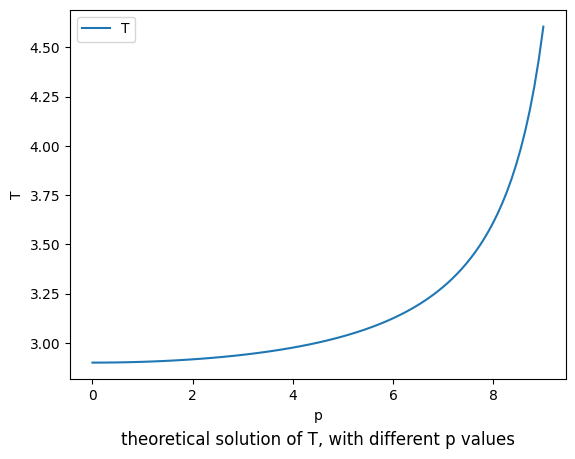
\includegraphics[width=10cm]{theory_T_diff_p.png}}
	\caption{The theoretical optimal T values against p values in the uncertainty set, from the formulation \ref{eq_Theory_T}}
	\label{theory_T_diff_p}
\end{figure}



Our rocket car problem is a typical bang-bang control problem, its optimal solution is obtained when the trajectory takes the extreme points whenever possible. This means acceleration, speed and deceleration take the maximum value whenever possible. A more proof of general bang-bang control problem needs the background knowledge in calculus of variations, Hamilton–Jacobi–Bellman equation, and the Pontryagin Maximum Principle etc. The paper \cite{KM16} gives a proof and explanation of the solution to the bang bang problem within a bilevel OCP. We refrain from diving deep into these theories, readers can refer to papers \cite{EJ89}, \cite{RV99} and \cite{BD05} for more information. 
 
The theoretical solution (equations \ref{eq_Theory_T} and \ref{eq_Theory_u}) to our problem \ref{rc} can also be obtained by solving the underlying partial differential equation \ref{rc_partial} directly, whiling taking the constraints into consideration. The proof are given in Appendix B of \cite{MatSch22}. The proof is tedious in detail, yet the underlying idea is simple and straightforward. Here we will briefly explain the idea behind the proof given in the paper \cite{MatSch22} and show with one example that the theoretical solution in formulation \ref{eq_Theory_T} and \ref{eq_Theory_u} is indeed correct. We take a fixed parameter value $p=0$ as an example for the explanation.

Because the objective is to minimize the time between the starting state and ending state, then it is optimal to run at the maximum allowable speed whenever possible, i.e with $x_2 =4$ as in the constraint \ref{rc_x2_tc}. Otherwise, time is wasted if a car is running at a speed that is less than the maximum allowable speed, i.e. $x_2=4$. Since the starting state is at position $0$ and speed $0$, to reach the maximum allowable speed as soon as possible, the car should be accelerated as strongly as possible at the begining until the speed reaches $x_2 =4$. Then the car should be running at this maximum speed for a certain period. After this period, the car should be decelerated as strongly as possible until the speed decreases to $0$, and exactly at the moment that the speed reaches $0$, the position should reach $10$. It is this moment that the optimal/smallest $T$ is achieved. How long the period should be running at maximum speed, depends on the acceleration/deceleration distance, which in turn depends on  starting/ending position (in our case, it is $0$ and $10$ respectively) and starting/ending speed (in our case, both are $0$). 

\begin{figure}[h]
	\centerline{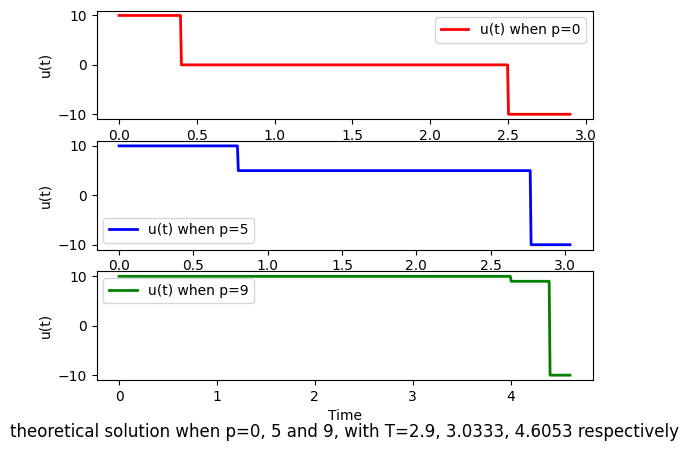
\includegraphics[width=10cm]{theory_ut_3p.png}}
	\caption{The theoretical u(t) values when p=0, p=5 and p=9, from the formulation \ref{eq_Theory_u}}
	\label{theory_ut_3p}
\end{figure}

This is a qualitative explanation why the solution from formulation \ref{eq_Theory_T} and \ref{eq_Theory_u} is correct. Now, we show that with $p=0$, the optimal time $T=2.9$. At the beginning $\tau_0 = 0$,  we should accelerate as much as possible until the real time $\tau_1=0.4$ (i.e. $t= \frac{\tau}{T} = 0.137931$). This number $\tau_1=0.4$ can be obtained by solving the partial differential equation \ref{rc_partial} with boundary conditions $x_2(\tau_0)=0$ and $x_2(\tau_1)=4$. At $\tau_1=0.4$, the car speed reaches $4$, and it keeps running at this speed $x_2=4$ till $\tau_2=2.5$. From $\tau=2.5$, the car starts to decelerate as strongly as possible, and at $T=\tau_3=2.9$, the speed reaches $0$ and the total distance traveled is exactly $10$. Then all the contraints are satisfied, and the optimal time is $T=2.9$. 

We can prove that $T=2.9$ is indeed the optimal solution when $p=0$ by using the method proof by contradiction. In the optimal strategy above, it has three stages $[\tau_0, \tau_1]$, $[\tau_1, \tau_2]$, and $[\tau_2, \tau_3]$, corresponding to acceleration, constant and deceleration stages. We assume there is another strategy that differs the one we have described above, yet leading to a less time while satisfying all the constraints. First, we assume the alternative strategy does not speed as strong as possible, this means within this alternative strategy, the speed of the car is always less or equal to the speed of our optimal strategy before $\tau_1=0.4$. This means that before $\tau_1=0.4$, the travel distance in the alternative strategy is less than our optimal strategy, and therefore, it will takes more time for car to cover the remaining distance in the alternative strategy. This alternative strategy, therefore, can not take less time compared to the optimal strategy. Similarly, we can prove that any modication to the optimal strategy will lead a bigger $T$ value. Therefore, by using the example of $p=0$, we have shown the solution \ref{eq_Theory_T} and \ref{eq_Theory_u} is indeed optimal with respect to different $p$ for all the $p$ in the uncertainty set $ \mathbb{P}=[p_l, p_u] =[0,9]$. The details of such proof can be found in paper \cite{MatSch22}. 

We can also numerically verified that the theoretical solution is correct. First, we show the theoretical solution of $T$ against different $p$ values accross the whole uncertainty set $\subset \mathbb{P} = [0,9]$, as shown in Figure \ref{theory_T_diff_p}. Then, we remove the uncertainty by showing the solution to the original problem \ref{rc} for several chosen $p_i$ values, where $ p_i  \in [p_0, p_1, ..., p_n] \subset \mathbb{P} = [0,9]$, here, we have chosen $p=0$,  $p=5$,  and $p=9$ as the example for illustration.  The $T$ values (rounded to four decimals) and the theoretical  $u(t)$ values corresponding to $p=0$,  $p=5$,  and $p=9$, are shown in Figure \ref{theory_ut_3p}. 

When $p$ takes fixed values, the OCP under uncertainty becomes a normal OCP problem and we can solve directly with the numerical methods discussed in Chapter \ref{Chapter2}, and no classical or training approach is needed. With $[0,1]$ discretized into $500$ subintervals $\mathbb{I}_j = [\tau_{j-1}, \tau_j]$, i.e. the discretizion points as $0 = t_0 =  < t_1 < ... < t_m = t_f =1 $, and an error tolerance level as $1e-6$, and Runge-Kutta RK4 method used,  the result from solving a normal OCP with $p=0$, $p=5$ and $p=9$ are shown in Figure \ref{fig1_org_u10_p0}, Figure \ref{fig1_org_u10_p5} and Figure \ref{fig1_org_u10_p9} respectively. 

Based on these three Figures \ref{fig1_org_u10_p0},  \ref{fig1_org_u10_p5} and \ref{fig1_org_u10_p9}, the results from $p=0$,  $p=5$,  and $p=9$ are consistent with that from the theoretical results in formulation \ref{eq_Theory_T} and \ref{eq_Theory_u}, as shown in Figure \ref{theory_T_diff_p} and Figure \ref{theory_ut_3p}. This confirms two points: first, the theoretical results are correct and second, the numerical methods we have chosen can solve our rocket car case with one chosen fixed $p$ value. These methods can, therefore, be used to solve general OCPs.

\begin{figure}[H]
	\centerline{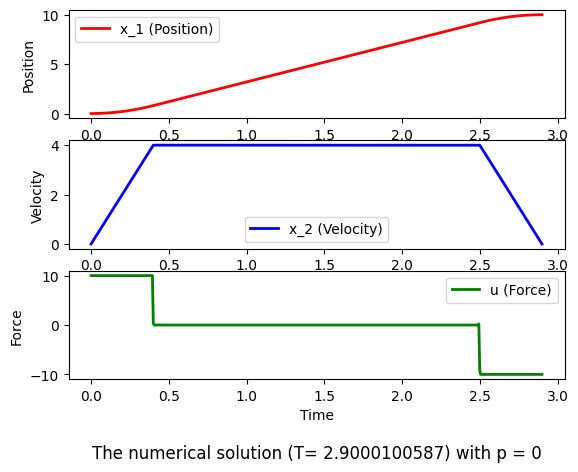
\includegraphics[width=10cm]{original_u10_p0.png}}
	\caption{Orginal rocket car problem \ref{rc} solution when p=0}
	\label{fig1_org_u10_p0}
\end{figure}

\begin{figure}[H]
	\centerline{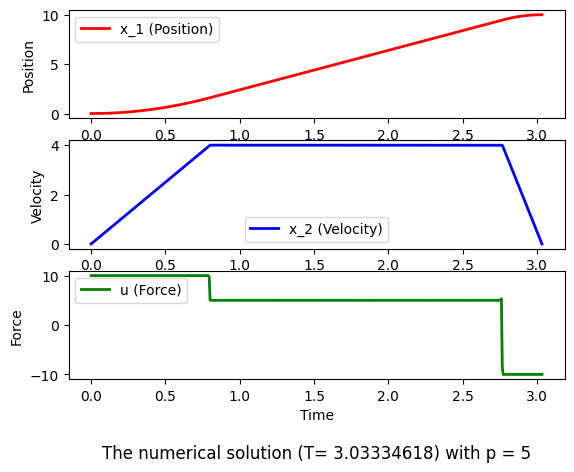
\includegraphics[width=10cm]{original_u10_p5.png}}
	\caption{Orginal rocket car problem \ref{rc} solution when p=5}
	\label{fig1_org_u10_p5}
\end{figure}

\begin{figure}[H]
	\centerline{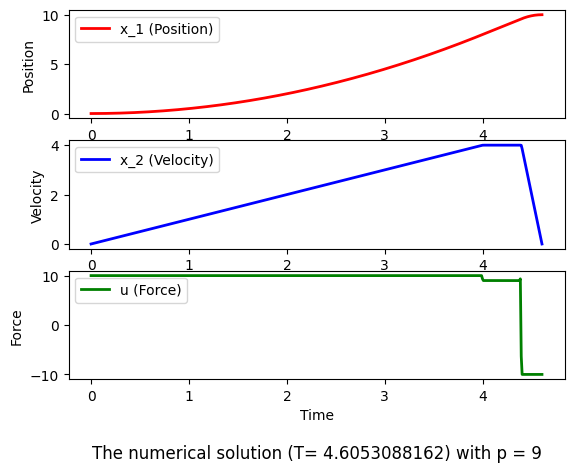
\includegraphics[width=10cm]{original_u10_p9.png}}
	\caption{Orginal rocket car problem \ref{rc} solution when p=9}
	\label{fig1_org_u10_p9}
\end{figure}

% By ananlyzing the optimal strHere we discuss several strategies. First assume at the ve
% and the ending state must be at a position larger than $10$ and speed smaller than $0$. To reach the maximum speed, from the starting state, we should accelerate as fast as possible until we reach the speed of $x_2 =4$, and then keep the car running at this speed until we need to decelerate as strongly as possible. The moment we start to decelerate is decided by how fast we can decelerate the speed decreases to exact $0$ is just the moment that the position reaches
%The proof is very tedious, but the idea is straightforward.

Because of the simplicity of the rocket car case, we can find the theoretical solution of the nominal/original problem for our case \ref{rc}. But for many real life problems, it is very difficult to find a direct solution to the original problem, and for some cases not feasible, due to the uncertainty in the parameter $p$. That is why in the paper \cite{MatSch22}, a classical (in the form $minmax$) approach and a training (in the form $maxmin$) approach have been discussed, and both approaches will lead to a conservative solution to the original problem. A conservative solution to the problem in the paper \cite{MatSch22}, or to general problems,  is a acceptable (or desired) result since less risk is taken and the result is more robust. In the next chapter, we discuss, in details, the classical approach and training approach for the rocket car problem. %After that, we focus on the quasi-Newton and multi shooting approach to the same problem.  

For both the classical approach and the training approach, after the discretization of the uncertainty set, the problem to be solved becomes a normal optimal control problem and we can use the mutiple shooting and quasi Newton (in the SQP framework) method to solve. We are levaraging open source package Casadi\footnote{Please refer the website https://web.casadi.org for more details} and Gekko\footnote{Please refer the website https://gekko.readthedocs.io/en/latest/ for more information} to solve our problem. These two package can let the user choose different nonlinear programming solver and as well as different underlying numerical methods. In our case, we have chosen the mutiple shooting and sequential quadratic programming, together with Runge–Kutta RK4 method. The numerical result from the classical approach and training approach will be discussed in the next two sections. 

\section{Apply classical (minmax) approach}
We have explained in Section \ref{Sec:CA} about the classical appraoch. Within this section, we further explain how this classical approach can be used for the chosen case. 
% Applying the classical approach to the rocket car case, the problem can be solved as follows. 

First we discretize the whole uncertainty set  $\mathbb{P}$ into multiple points in an increasing order $[p_0, p_1, ..., p_n] \subset \mathbb{P}$ so that $p_i, i =0, 1, ..., n$ can approximately representing the whole set $\mathbb{P}$ when $n$ is large enough. Here $p_0=p_l$ and $p_n= p_u$, with $[p_l, p_u] =[0,9]$, as shown in equation \ref{uncertainP}.  We solve the $minmax$ problem of the following form
\begin{subequations}
	\begin{align}
		\underset{\epsilon, u(\cdot), x(\cdot)}{min}  \ \   &  \underset{p_i \in \mathbb{P}}{max}  \  \epsilon \\ 
		s.t.  &  \ \ T  \leq \epsilon \\
		&  \ \ x = (x_1, x_2),   \label{ca_rc_x} \\ 
		& \ \  \dot{x} = T  \begin{pmatrix}  x_2(t;p_i) \\ u(t)-p_i   \end{pmatrix}, &  \ \forall \   p_i, \  t \in [0,1],  \label{ca_rc_partial} \\
		& \ \ x(0,p_i) = 0, \label{ca_rc_t0}\\
		& \ \ x_1(1;p_i) \geq 10  & \ \forall \   p_i,   \label{ca_rc_x1_t1} \\
		& \ \ x_2(t;p_i) \leq 4, &   \ \forall \   p_i,  t \in [0,1] \label{ca_rc_x2_tc} \\
		& \ \ x_2(1;p_i) \leq 0,   & \ \forall \   p_i,  \label{ca_rc_x2_t1}  \\
		& \ \ T \geq 0, \\
		& \ \ u(t) \in [-10, 10], & \ \ t \in [0,1]. 
	\end{align}
	\label{ca_rc}
\end{subequations}
for all $p_i$ where $p_i \in [p_0, p_1, ..., p_n] \subset \mathbb{P}$. Since both $u(\cdot)$ and $x(\cdot)$ are functions of $t$, we also needs to discretize these two varaibles in the time horizon. In this classical approach, the driver has no prior knowledge about the value of the parameter $p$ and gets no feedback during the process and has to set up the driving strategy in advance. The realization of the trajectory of $u(\cdot)$ and $x(\cdot)$ may not be an optimal solution with any given $p$ value. 
In the end, we get solutions of $x$, $u$ and $ \epsilon$ which are conservative to all the $p_i \in \mathbb{P}$, and does not depend on any parameter $p$. 

In the actual implementation, we have take $n=40$, i.e. in total $40 \ p_i$ points ranging the whole uncertainty set $\mathbb{P}=[0,9]$, but here in the graph, we show the result only for $p=0, 1, 2, 3, 4, 5, 6, 7, 8, 9$

Numerical result to be added for the classical approach.  

%where $p_i$ is one of the discretized point $p_0, p_1, ..., p_n$  from the  $\mathbb{P}$. Therefore, for each $ p_i \in \mathbb{P}$, we get a corresponding solution. In the end, we get a robustified parameter-dependent varaibles for realizations of the unceretain parameters. The bigger the number $n$, i.e. the more points of $p_i$, the more precise that the obtained solution can represent the whole uncertain set. In this classical approach, the driver has no prior knowledge about the value of the parameter $p$ and gets no feedback during the process and has to set up the driving strategy in advance. The numerical implementation result of the classical approach is shown in section \ref{Sec_NR} when comparing that of the training approach. 

% \ \forall \   \hat{p}_i,
%As stated in the introduction part, the classical approach is consistent with the $minmax$ approach, during which, two level optimization problems are solved. In the lower level, we solve an optimization problem ($max \  f(x,p)$) with respect to $p$, and in the upper level, we continue to find the best solution with respect to $x$, as shown in \ref{minmax}. In the case of the rocket car, the classical approach will be expressed in the following form

%In the classical approach, the set of feasible controllable parameters and control functions are given by those $T$ and $u(\cdot)$, which yield feasible trajectories $x(\cdot, p)$ for all $p \in \mathbb{P}$. The value of the objective function in the lower level does not depend on $p$ and $x(\cdot, p)$. In other words, in this approach, the driver has no prior knowledge about the value of the parameter $p$ and gets no feedback during the process and has to set up the driving strategy in advance.  

% \section{The Training Approach}

\section{Apply training (maxmin) approach}
Contrast to the classical approach, in the training approach it is assumed that the driver of the rocket car is able to perform optimally for every $p$ because of a preceding training period. We discretize the uncertainty set $\mathbb{P}$ the same as in the classical approach, i.e. we take the discretized points $p_0, p_1, ..., p_n$ which cover the whole uncertainty set $\mathbb{P}$.  For each $ p_i  \in [p_0, p_1, ..., p_n] \subset \mathbb{P}$, we solve the problem 
\begin{subequations}
	\begin{align}
		 \underset{p_i \in \mathbb{P}}{max}  \ \underset{T, u(\cdot), x(\cdot)}{min}  \ \   &   T  \\ 
		s.t.  & \ \ x = (x_1, x_2),   \label{ta_rc_x} \\ 
		& \ \  \dot{x} = T  \begin{pmatrix}  x_2(t;p_i) \\ u(t)-p_i   \end{pmatrix}, & \ t \in [0,1],  \label{ta_rc_partial} \\
		& \ \ x(0,p) = 0, \label{ta_rc_t0}\\
		& \ \ x_1(1;p_i) \geq 10, \label{ta_rc_x1_t1} \\
		& \ \ x_2(t;p_i) \leq 4, & t \in [0,1], \label{ta_rc_x2_tc} \\
		& \ \ x_2(1;p_i) \leq 0, \label{ta_rc_x2_t1}  \\
		& \ \ T \geq 0, \\
		& \ \ u(t) \in [-10, 10], & t \in [0,1]. 
	\end{align}
	\label{TA_rc}
\end{subequations}
With a given $p_i$ value, the lower level optimization problem turns out to be a normal OCP. One $p_i$ value will correspond to one optimal $T_i$ values. Among all the optimal $T_i$, we would like to find the worst case, i.e. the largest among all $T_i$ values. Similar to the discretization of the uncertainty set in the classical approach, here we also take $n=40$, i.e. in total $40 p_i$ points ranging the whole uncertainty set $\mathbb{P}=[0,9]$.  The result of $T_i$ against $p_i$ is shown in Figure \ref{fig_ta_numerical_T_p}.  Figure \ref{fig_ta_numerical_T_p} is almost indentical to Figure \ref{theory_T_diff_p}, which confirms again that our numerical result with different $p$ is consistent with the theoretical result. Furthermore, the worst case over all $p_i$ is when $p_i$ takes the biggest value, i.e. $p_i =9$, and in this case $T_i = 4.6053$.  We already shown in Figure \ref{fig1_org_u10_p9} the solution to original problem when $p_i=9$. The worst case, therefore, have the same solution as shown in Figure \ref{fig1_org_u10_p9}, with  $T=4.6053$, which we do not repeat here. 
\begin{figure}[h]
	\centerline{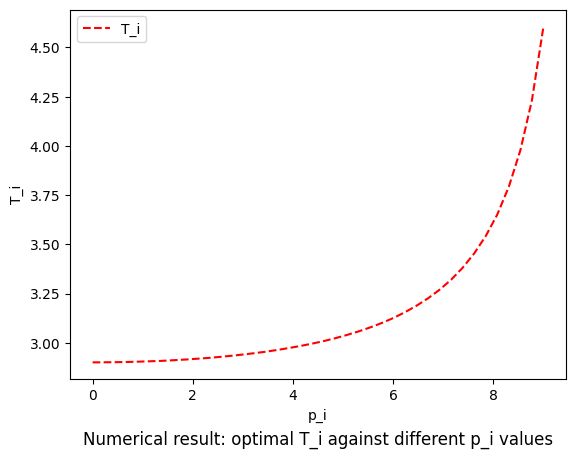
\includegraphics[width=10cm]{numerical_T_p.png}}
	\caption{Numerical result: different $T_i$ values against different $p_i$ values, with $p_i=9$ and  $T_i=4.6053$ the worst case}
	\label{fig_ta_numerical_T_p}
\end{figure}

%From analyzing the theoretical solution, 
%The solution of the training approach in this paper is, therefore, also a function of the realizations of the uncertain parameters. Since in the 
 %The numerical result will be shown in the next section \ref{Sec_NR}.

\section{Analysis the numerical results}
\label{Sec_NR}



%Before we discuss the results from the classic approach and training approach, we discuss our primary analysis of the original problem \ref{rc}. 

%We can further prove the theoretical solution in formulation \ref{eq_Theory_T} and \ref{eq_Theory_u} by showing the following facts. First, with more time steps



%When we plot the optimal $T$ against the uncertain parameter $p$, then we get the result in Figure  

%The implementation deatils and result are as follows. 
%\begin{figure}[h!]
%	\centerline{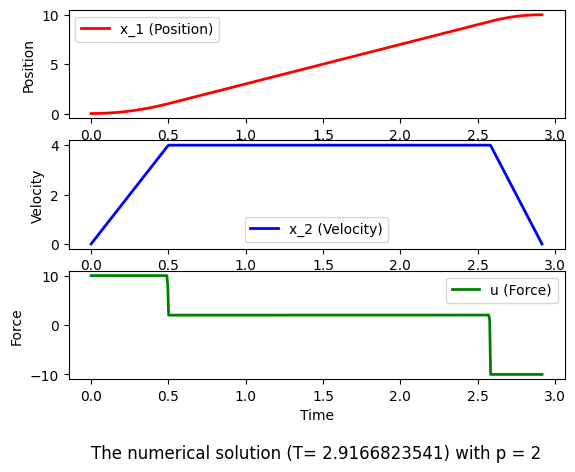
\includegraphics[width=10cm]{original_u10_p2.png}}
%	\caption{price and delta from three different methods}
%	\label{fig:result}
%\end{figure}
%\begin{figure}[h!]
%	\centerline{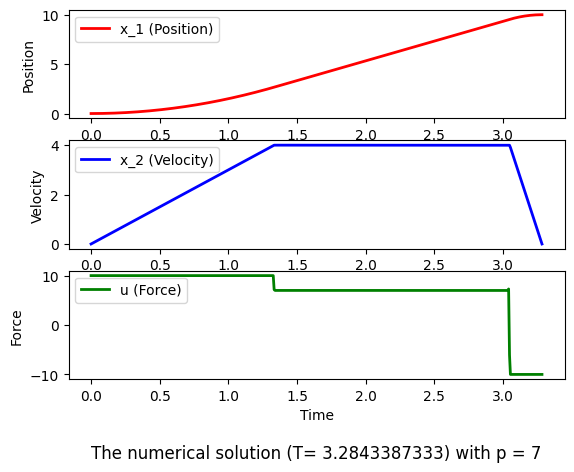
\includegraphics[width=10cm]{original_u10_p7.png}}
%	\caption{price and delta from three different methods}
%	\label{fig:result}
%\end{figure}



\chapter{Conclusion}
\label{Chapter5}

 
 %where $p^0$ is a fixed value in the feasible uncertainty set $\Omega_P$, where the parameter $p$ can take value from.In the paper \cite{MatSch22}, multiple methods of solving the parameterized optimization problem have been discussed. The main focus (of solving the Cerebral Palsy problem) of the paper \cite{MatSch22}, is the "worst-case treatment planning by bilevel optimal control", i.e. a bilevel optimization problem. The bilevel optimisation method in paper \cite{MatSch22} solves the parameterized optimization problems, e.g. the Cerebral Palsy problem, in a conservative way.One method of solving the original CP problem in a conservative way is to transform the problem \ref{ParaMin} into another form. 
 
 %Based on theorem \ref{TH_KKT}, We want to solve equation \ref{eq:GradientLagrange}.
 %\begin{align}
 %	\label{eq:GradientLagrange}
 %	\nabla 	\mathcal{L}(w,\lambda, \mu) = 0.
 %\end{align}
 %where its derivatives is as follows
 %\begin{equation}
 %\begin{align}
 %	\nabla \mathcal{L}(w,\lambda, \mu) &= 
 %	\mtrx{
 	%		\nabla_w f(w) +  \nabla_w g(w) \lambda + \nabla_w h(w) \mu  \\
 	%		g(w)    \\
 	%		h(w)
 	%	} 
 %\end{align}
 
 %	\nabla^2 \mathcal{L}(w,\lambda, \mu) &=
 %\mtrx{
 	%	\nabla^2_w f(w) + \nabla^2_w g(w)\lambda  & \nabla_w g(w) & \nabla_w h(w)\\
 	%	\nabla_w g(w) ^\top\\
 	%	\nabla_w h(w)^\top
 	%}
 
 
 %\end{equation}
 % 	\mathcal{L}(w,\lambda, \mu) &= \Phi(w) - \lambda ^\top a(w)-  \mu^\top b(w) \\
 
 
 
 
 %We apply Newton's method and we have to solve for $(w_i,\lambda_i, \mu_i)$ :
 %\begin{align}
 %	\nabla^2 \mathcal{L}(w_i,\lambda_i, \mu_i) \Delta w +  \nabla \mathcal{L}(w_i,\lambda_i, \mu_i) = 0.
 %\end{align}
 
 %Equivalently, the following QP ( Quadratic Programming ) needs to be solved:
 
 
 
 
 % and include the equality
 %\begin{equation}
 %	\mathcal{L}(x,\lambda, \mu) = f(x) + \lambda^\top g(x) +  \mu^\top h(x) 
 %	\label{eq_Lagrangian}
 %\end{equation}
 
 
 
 
 %The optimal control problem (OCP) \ref{P2_OPM} involves constraints in the partial differential equation form and in a time horizon $t \in [t_0, t_f]$. Therefore, we can apply multiple shooting method discretize the original OCP of the whole interval into mutiple OCPs in different subintervals, with the constraints enforced at the boundary of subintervals to guarantee the continuity. Together with the matching conditions, we can then aggregate the subproblems and apply quasi Newton method to get the final optimal solution. The numerical solution, with multilpe shooting and quasi Newton method to solve optimal control problem, will be demnostrated with rocket car case in Chapter \ref{Chapter4}.  
 
 %In the next section, we explain the multilpe shooting method first and in the next chapter we then focus on how th




%The constrained optimization \ref{eq:OCP_discret_compact} can form the Lagrangian function
%\begin{equation}
%	 \mathcal{L}(w,\lambda, \mu) = \Phi(w) - \lambda ^\top a(w)-  \mu^\top b(w) 
%\end{equation}


%\definition (Active Constraints and Active Set) An inequality constraint hi(x) ≤ 0 is called active at x∗ 2 Ω
%iff hi(x∗) = 0 and otherwise inactive. The index set A(x∗) ⊂ f1; : : : ; nhg of active inequality constraint indices
%is called the ”active set”




%The Karush–Kuhn–Tucker theorem then states the following.


%% = \frac{x_2(t_k) + x_2(t_{k-1})}{2} (\tau_k -\tau_{k_1})
%%%  \frac{x_2(t_k) + x_2(t_{k-1})}{2} (\tau_k -\tau_{k_1}) 
   
   
   
   
   
   
   % t&= \frac{\tau}{T} \in [0,1] \quad \tau \in [0, T]
   %\\
   %i.e. \ \begin{pmatrix} \dot{x_1} \\ \dot{x_2} \end{pmatrix} &= \begin{pmatrix} \frac{\partial x_1}{\partial t} \\ \frac{\partial x_2}{\partial t} \end{pmatrix} = 
   %\begin{pmatrix} \frac{\partial x_1}{\partial \tau} \frac{\partial \tau}{\partial t}  \\ \frac{\partial x_2}{\partial \tau} \frac{\partial \tau}{\partial t} \end{pmatrix} 
   
   %\begin{equation*}
   %	\begin{align}
   %		\dot{x} =  \begin{pmatrix} \dot{x_1} \\ \dot{x_2} \end{pmatrix}  & =  T  \begin{pmatrix}  x_2(t;p) \\ u(t)-p   \end{pmatrix} = \begin{pmatrix}  Tx_2(t;p) \\ T(u(t)-p)   \end{pmatrix} \\
   %		i.e. \ \begin{pmatrix} \dot{x_1} \\ \dot{x_2} \end{pmatrix} &= \begin{pmatrix} \frac{\partial x_1}{\partial t} \\ \frac{\partial x_2}{\partial t} \end{pmatrix} = 
   %		\begin{pmatrix} \frac{\partial x_1}{\partial \tau} \frac{\partial \tau}{\partial t}  \\ \frac{\partial x_2}{\partial \tau} \frac{\partial \tau}{\partial t} \end{pmatrix} 
   %	\end{align}
   %\end{equation*}
   
   
   
   
   
   
   
   
   \newpage
  \part{Appendix}
  \begin{appendix}
    \chapter{Lists}
    %\listoffigures
    %\listoftables
    \bibliography{references}{}
    \citestyle{egu}
    \bibliographystyle{plainnat}
    \setlength{\parindent}{0em}

Erkl\"{a}rung:\par
\vspace{3\baselineskip}
Ich versichere, dass ich diese Arbeit selbstst\"{a}ndig verfasst habe und keine
anderen als die angegebenen Quellen und Hilfsmittel benutzt habe.\par
\vspace{5\baselineskip}
Heidelberg, den (Datum)\hspace{3cm}\dotfill
%
\vspace{8\baselineskip}

Declaration:\par
\vspace{3\baselineskip}
I hereby confirm that I wrote this work independently and did not use any sources other than those indicated.\par
\vspace{5\baselineskip}
Heidelberg, (Date)\hspace{3cm}\dotfill



  \end{appendix}
\end{document}

   %

\chapter{The Classical and Training Approach}

The paper on hand focuses on using quasi-Newton and multi-shooting method for the Training Approach. In this chapter, we shortly introduce the Classical Approach first and then we discuss the Training Approach in greater detail. In the next chapter, we can introduce the quasi-Newton and multi-shooting method, and elaborate in detail how they can be used for the Training Approach. 



\section{The Classical Approach}

As stated in the introduction part, the classical approach is consistent with the $minmax$ approach, during which, two level optimization problems are solved. 

In the lower level, we solve an optimization problem ($max \  f(x,p)$) with respect to $p$, and in the upper level, we continue to find the best solution with respect to $x$, as shown in \ref{minmax}. In the case of the rocket car, the classical approach will be expressed in the following form

\begin{subequations}
	\begin{align}
		\underset{T, u(\cdot)}{min} \  \underset{ p \in \Omega_P, x(\cdot,p)}{max}  \ \   & \  T \\ 
		s.t.  & \ \ x = (x_1, x_2)   \label{ca_rc_x} \\ 
		& \ \  \dot{x} = T  \begin{pmatrix}  x_2(t;p) \\ u(t)-p   \end{pmatrix}, & \ t \in [0,1],  \label{ca_rc_partial} \\
		& \ \ x(0,p) = 0, \label{ca_rc_t0}\\
		& \ \ x_1(1;p) \geq 10, & \ for \ all \ p \in \Omega_P, \label{ca_rc_x1_t1} \\
		& \ \ x_2(t;p) \leq 4, & t \in [0,1], \ for \ all \ p \in \Omega_P,  \label{ca_rc_x2_tc} \\
		& \ \ x_2(1;p) \leq 0, & \ for \ all \ p \in \Omega_P, \label{ca_rc_x2_t1}  \\
		& \ \ T \geq 0, \\
		& \ \ u(t) \in [-10, 10], & t \in [0,1]. 
	\end{align}
	\label{ca_rc}
\end{subequations}

In the Classical Approach, the set of feasible controllable parameters and control functions are given by those $T$ and $u(\cdot)$, which yield feasible trajectories $x(\cdot, p)$ for all $p \in \Omega_P$. The value of the objective function in the lower level does not depend on $p$ and $x(\cdot, p)$. In other words, in this approach, the driver has no prior knowledge about the value of the parameter $p$ and gets no feedback during the process and has to set up the driving strategy in advance. 

\section{The Training Approach}
Contrast to the Classical Approach, in the Training Approach it is assumed that the driver of the rocket car is able to perform optmially for every $p$ because of a preceding training period. Thus the worst possible optimal performance is given by a solution of the problem
\begin{subequations}
	\begin{align}
	   \underset{p \in \Omega_P, T, u(\cdot), x(\cdot,p)}{max}  \ 	\underset{}{min} \   & \  T \\ 
		s.t.  & \ \ x = (x_1, x_2)   \label{ta_rc_x} \\ 
             & \ \  \dot{x} = T  \begin{pmatrix}  x_2(t;p) \\ u(t)-p   \end{pmatrix}, & \ t \in [0,1],  \label{ta_rc_partial} \\
& \ \ x(0,p) = 0, \label{ta_rc_t0}\\
& \ \ x_1(1;p) \geq 10, \label{ta_rc_x1_t1} \\
& \ \ x_2(t;p) \leq 4, & t \in [0,1], \label{ta_rc_x2_tc} \\
& \ \ x_2(1;p) \leq 0, \label{ta_rc_x2_t1}  \\
& \ \ T \geq 0, \\
& \ \ u(t) \in [-10, 10], & t \in [0,1]. 
	\end{align}
	\label{TA_rc}
\end{subequations}

The solution of the Training Approach in paper \cite{MatSch22} is given by a gradient-free method, more precisely, a so-called model-based DFO approach for box-constrained optimization problems is used. The BOBYQA algorithm is chosen for such approach to solve problems of the form
\begin{equation}
	\begin{aligned}
		\underset{x \in \mathcal{R}^n}{min} & \  F(x)  \\ 
		s.t.  & \ a_i \leq x_i \leq b_i, i = 1, ..., n \\
	\end{aligned}
	\label{DFO_bc}
\end{equation}

The name BOBYQA is an acronym for "Bound Optimization BY Quadratic Approximation", and is used to solve lower level problem of \ref{TA_rc}. In the general DFO method, the objective function $F(\cdot)$ is considered a black box. For a given $p$, the parametric lower level OCP is solved with a direct approach and the resulting (finite dimensional) solution is viewed as dependent variable. Furthermore, the uncentainty set $\Omega_P$ is box-shaped, and hence the BOBYQA algorithm is applicable to the problem in the Training Approach.The BOBYQA algorithm has been introduced in details in the paper \cite{MicPow22}, and we reiterate the main idea in the text that follows.  

The method of BOBYQA is iterative, $k$ and $n$ being reserved for the iteration number and the number of variables, respectively. Further, $m$ is reserved for the number of interpolation conditions that are imposed on a quadratic approximation $Q_k(x), x \in \mathcal{R}$, to $F(x), \mathcal{R}$, with $m$ is a chosen constant  integer from the interval $[n+2, \frac{1}{2}(n+1)(n+2)]$. The approximation is available at the beginning of the $k$-th iteration, the interpolation equations have the form
\begin{equation}
  Q_k(y_j)= F(y_j),\   j = 1, 2, ..., m, 
\end{equation}
We let $x_k$ be the point in the set $\{y_j : j = 1, 2, ... , m\}$ that has the property
\begin{equation}
	F(x_k)= min\ \{F(y_j), \  j = 1, 2, ..., m\}, 
\end{equation}
with any ties being broken by giving priority to an earlier evaluation of the least function value $F(x_k)$. A positive number $\Delta_k$, called the “trust region radius”, is also available at the beginning of the $k$-th iteration. If a termination conditions is satisfied, then the iteration stops. Otherwise, a step $d_k$ from $x_k$ is constructed such 
that $ \Vert d_k \Vert \leq \Delta_k $ holds, such that $x = x_k+d_k$ is within the bounds \ref{DFO_bc}, and such that $x_k+d_k$ is not one of the interpolation points $y_j : j = 1, 2, ... , m$. Then the new function value $F(x_k+d_k)$ is calculated, and one of the interpolation points, $y_t$ say, is replaced by $x_k+d_k$, where $y_t$ is different from $x_k$. It follows that $x_{k+1}$ is defined by the formula
\begin{equation}
	x_{k+1}
	\begin{cases}
		 x_k, & F(x_k+d_k) \geq F(x_k) \\
		x_k+d_k  , & F(x_k+d_k) < F(x_k) 
	\end{cases}
\end{equation}

Further, $\Delta_{k+1}$ and $Q_{k+1}$ are generated for the next iteration, $Q_{k+1}$ being subject to the constraints 
\begin{equation}
	Q_{k+1}(\hat{y}_j)= F(\hat{y}_j), \  j = 1, 2, ..., m, 
\end{equation}
at the new interpolation points
\begin{equation}
	\hat{y}_j =
	\begin{cases}
		y_j, & j \neq t, \\
		x_k+d_k  , & j =t 
	\end{cases},  \  j = 1, 2, ..., m.
\end{equation}


%In the method of BOBYQA algorithm, in each iteration $k$ the objective function is approximated by a sequence of quadratic function $Q_k(\cdot)$, such that 
%\begin{equation}
%	\begin{aligned}
%Q_k(z^{k,i}) = F(z{k,i}), \   i = 1, ..., m,
%	\end{aligned}
%	\label{BOBYQA}
%\end{equation}
%for interpolation points $z^{k,i} \in \mathcal{R}$. The number of interpolation points $m$ is constant. Let $x_k \in \ argmin \ \{Q_k(z^{k,i}) | i=1, ...,m\}$. In every iteration $k$, by means of quadrative model, one computes a feasible step $d_k$, which is inside a "trust-region radius" $\Delta_k$, i.e. $\l d_k \leq \Delta_k$. Subsequently, the function $F(\cdot)$ is evaluated at $x_k + d_k$, one interpolation point $z^{k,i}$ is replaced by $x_k + d_k$, and the quadrative model is updated. The sequence $x_k$ is expected to approach a solution of Problem \ref{DFO_bc}.

 











%can assume that $p^0$ is a fixed value in the feasible uncertainty set $\Omega_P$

%The classical approach, aka, the robust optimization  is concerned with optimization problems which involes uncertainy parameters whose value is a priori unknown. 


% approach and the
%

\chapter{The Introduction to Multiple Shooting and Quasi-Newton Method}

In this chapter, we first introduce the basics of solutions to nonlinear problems and the focus on the quasi-Newton and multiple shooting method. 

As stated in the introduction chapter \ref{Chapter1}, a general optimization problem is typically of the form 
\begin{equation}
	\begin{aligned}
		\  \  \ & min \  f(x) \\
		s.t.\ \  & x \in \Omega
	\end{aligned}
	\label{GeneralOpt}
\end{equation}

Here $x \in \Omega$ represents the constraints for which $x$ must satisfy, it may be in the form of $ g(x) = 0,  h(x)  \geq  0$ as in the problem \ref{GeneralMin} in the Introduction chapter, i.e. the feasible set $\Omega = \underset{x}{arg} \ \{ g(x) = 0,  h(x)  \geq  0 \}$. 

Such problem can be solved via Newton's method, which attempts to solve this problem by constructing a sequence $\{x_K\}$ from an initial guess (starting point) $x_0 \in \Omega$ that converges towards a minimizer $x^\star$ of $f(x)$  by using a sequence of first and/or second order Taylor approximations of $f(x)$ around the iterates. The second-order Taylor expansion of $f(x)$ around $x_k$ is
%\begin{multline*}
\begin{align*}
f(x_k + \delta_x) \approx f(x_k) + f'(x_k)\delta x +\frac{1}{2}f''(x_k)\delta_x^2
\end{align*}
where $\delta_x$ represents a small change (with respect to $x$), and $f', f''$ are the first and second order derivatives of the original function $f(x)$. 
%\end{multline*}




%{\displaystyle f(x_{k}+t)\approx f(x_{k})+f'(x_{k})t+{\frac {1}{2}}f''(x_{k})t^{2}.}{\displaystyle f(x_{k}+t)\approx f(x_{k})+f'(x_{k})t+{\frac {1}{2}}f''(x_{k})t^{2}.}
%The next iterate {\displaystyle x_{k+1}}x_{k+1} is defined so as to minimize this quadratic approximation in {\displaystyle t}t, and setting {\displaystyle x_{k+1}=x_{k}+t}{\displaystyle x_{k+1}=x_{k}+t}. If the second derivative is positive, the quadratic approximation is a convex function of {\displaystyle t}t, and its minimum can be found by setting the derivative to zero. Since

%{\displaystyle \displaystyle 0={\frac {\rm {d}}{{\rm {d}}t}}\left(f(x_{k})+f'(x_{k})t+{\frac {1}{2}}f''(x_{k})t^{2}\right)=f'(x_{k})+f''(x_{k})t,}{\displaystyle \displaystyle 0={\frac {\rm {d}}{{\rm {d}}t}}\left(f(x_{k})+f'(x_{k})t+{\frac {1}{2}}f''(x_{k})t^{2}\right)=f'(x_{k})+f''(x_{k})t,}
%the minimum is achieved for

%{\displaystyle t=-{\frac {f'(x_{k})}{f''(x_{k})}}.}{\displaystyle t=-{\frac {f'(x_{k})}{f''(x_{k})}}.}
%Putting everything together, Newton's method performs the iteration

%{\displaystyle x_{k+1}=x_{k}+t=x_{k}-{\frac {f'(x_{k})}{f''(x_{k})}}.}{\displaystyle x_{k+1}=x_{k}+t=x_{k}-{\frac {f'(x_{k})}{f''(x_{k})}}.}

%Here, the function $f(x)$ is typically a non-linear function. 




%Without attempting completeness, we pr















%can assume that $p^0$ is a fixed value in the feasible uncertainty set $\Omega_P$

%The classical approach, aka, the robust optimization  is concerned with optimization problems which involes uncertainy parameters whose value is a priori unknown. 


% approach and the
%\chapter{Rocket Car Case}
Before we dive into the mathematics, we first re-introduce the physics of the rocket car case so that we can model the problem more precisely. Within the training approach, with a given $p$, we want to solve the lower level problem of the following form \ref{TA_lower}
\begin{subequations}
	\begin{align}
    	\underset{}{min} \   & \  T \\ 
		s.t.  & \ \ x = (x_1, x_2)   \label{ta_rc_x} \\ 
		& \ \  \dot{x} = T  \begin{pmatrix}  x_2(t;p) \\ u(t)-p   \end{pmatrix}, & \ t \in [0,1],  \label{ta_rc_partial2} \\
		& \ \ x(0,p) = 0, \label{ta_rc_t2}\\
		& \ \ x_1(1;p) \geq 10, \label{ta_rc_x1_t2} \\
		& \ \ x_2(t;p) \leq 4, & t \in [0,1], \label{ta_rc_x2_tc2} \\
		& \ \ x_2(1;p) \leq 0, \label{ta_rc_x2_t1_2}  \\
		& \ \ T \geq 0, \\
		& \ \ u(t) \in [-10, 10], & t \in [0,1], \\
		& \ \ p, \   a \ given \ value
	\end{align}
	\label{TA_lower2}
\end{subequations}

In summary, we want to find the minimum time that the rocket car moves from the starting state (the position is at the origin point, and the speed is zero) to an ending state when the position is at least at point 10 or beyond, and the speed is less than or equal to zero (a negative speed indicates the car is moving in a direction that decreases the position), with constraints on the acceleration/deceleration value and the speed during the whole process. 

Because our objective is to minimize the time between starting state and ending state, i.e. the variable $T$, which is unknown, we cannot define a time horizon over which we will discretize and optimize. Therefore, a new variable $t$ is defined as follows: 
\begin{equation*}
 	t= \frac{\tau}{T} \in [0,1] \quad \tau \in [0, T]
 	\label{eqn:timet}
\end{equation*}

Where $\tau$ is the real time between starting time $0$ and ending time $T$, and $t$ is the relative time between $0$ and $1$.  The equation \ref{ta_rc_partial2} can be also written as 

\begin{subequations}
		\begin{align}
 \dot{x} =  \begin{pmatrix} \dot{x_1} \\ \dot{x_2} \end{pmatrix}  & =  T  \begin{pmatrix}  x_2(t;p) \\ u(t)-p   \end{pmatrix} = \begin{pmatrix}  Tx_2(t;p) \\ T(u(t)-p)   \end{pmatrix} \label{eq_difT} \\ 
 \begin{pmatrix} \dot{x_1} \\ \dot{x_2} \end{pmatrix} &= \begin{pmatrix} \frac{\partial x_1}{\partial t} \\ \frac{\partial x_2}{\partial t} \end{pmatrix} = \begin{pmatrix} \frac{\partial x_1}{\partial \tau} \frac{\partial \tau}{\partial t} \\ \frac{\partial x_2}{\partial \tau} \frac{\partial \tau}{\partial t} \end{pmatrix} =  \begin{pmatrix} \frac{\partial x_1}{\partial \tau} T \\ \frac{\partial x_2}{\partial \tau}T \end{pmatrix} =     \begin{pmatrix}  Tx_2(t;p) \\ T(u(t)-p)   \end{pmatrix} \\
 \begin{pmatrix} \frac{\partial x_1}{\partial \tau}  \\ \frac{\partial x_2}{\partial \tau} \end{pmatrix} & =     \begin{pmatrix}  x_2(t;p) \\ (u(t)-p)   \end{pmatrix} \label{eq_difTau}
 	\end{align}
 \end{subequations}

In summary, the equation $\frac{\partial x_1}{\partial \tau}= x_2(t;p) $ means the change in the position in real time is proportional to the speed at that moment. And the equation $\frac{\partial x_2}{\partial \tau} = u(t)-p $ means the change in speed is proportional to the acceleration/deceleration value at that moment. 

To use multiple shooting and quasi-Newton method, we discretize the interval $t\in [0,1]$ into subinterval $[t_{k-1}, t_k], k = 1, 2, ..., m$, where $0 =t_0, t_1, t_2, ...,t_{k-1}, t_k, ..., t_m=1$. We solve the OCP within each interval, and enforce the matching condition at the boundary of each interval. 

The equation \ref{eq_difT} is equivalent to \ref{eq_difTau}





% t&= \frac{\tau}{T} \in [0,1] \quad \tau \in [0, T]
%\\
%i.e. \ \begin{pmatrix} \dot{x_1} \\ \dot{x_2} \end{pmatrix} &= \begin{pmatrix} \frac{\partial x_1}{\partial t} \\ \frac{\partial x_2}{\partial t} \end{pmatrix} = 
%\begin{pmatrix} \frac{\partial x_1}{\partial \tau} \frac{\partial \tau}{\partial t}  \\ \frac{\partial x_2}{\partial \tau} \frac{\partial \tau}{\partial t} \end{pmatrix} 

%\begin{equation*}
%	\begin{align}
%		\dot{x} =  \begin{pmatrix} \dot{x_1} \\ \dot{x_2} \end{pmatrix}  & =  T  \begin{pmatrix}  x_2(t;p) \\ u(t)-p   \end{pmatrix} = \begin{pmatrix}  Tx_2(t;p) \\ T(u(t)-p)   \end{pmatrix} \\
%		i.e. \ \begin{pmatrix} \dot{x_1} \\ \dot{x_2} \end{pmatrix} &= \begin{pmatrix} \frac{\partial x_1}{\partial t} \\ \frac{\partial x_2}{\partial t} \end{pmatrix} = 
%		\begin{pmatrix} \frac{\partial x_1}{\partial \tau} \frac{\partial \tau}{\partial t}  \\ \frac{\partial x_2}{\partial \tau} \frac{\partial \tau}{\partial t} \end{pmatrix} 
%	\end{align}
%\end{equation*}



 

%
% 

\chapter{Rocket car case}
Since the approaches we are going to use in this paper will be demonstrated with the case of rocket car, we decide to describe the rocket car case first. So that, when we are discussing our approaches, we can directly describe how they can be used in solving the rocket car case. The description of the rocket car case is mostly coming from the paper \cite{MatSch22}, with content either verbatim or in a modified form. 

We consider the rocket car case with state constraints, i.e. the one-dimensional movement of a mass point under the influence of some constant acceleration/deceleration, e.g. modeling head-wind or sliding friction, which can accelerate and decelerate in order to reach a desired position. The mass of the car is normalized to 1 unit\footnote{We do not specify the unit on purpose since the actual unit, either one kilogram or meter, does not play a role in the modeling. We are more concerned about the scale.} and the constant acceleration/deceleration enters the model in form of an unknown parameter $p \in \Omega_P \subset \mathbb{R}$ suffering from uncertainty, with the uncertainty set $\Omega_P$ convex and compact. We consider a problem in which the rocket car shall reach a final feasible position and velocity in a minimum time: 



\begin{subequations}
	\begin{align}
		\underset{T, u(\cdot), x(:,p)}{min} \   & \  T \\ 
		s.t.  & \ \ x = (x_1, x_2)   \label{rc_x} \\ 
		& \ \  \dot{x} = T  \begin{pmatrix}  x_2(t;p) \\ u(t)-p   \end{pmatrix}, & \ t \in [0,1],  \label{rc_partial} \\
		& \ \ x(0,p) = 0, \label{rc_t0}\\
		& \ \ x_1(1;p) \geq 10, \label{rc_x1_t1} \\
		& \ \ x_2(t;p) \leq 4, & t \in [0,1], \label{rc_x2_tc} \\
		& \ \ x_2(1;p) \leq 0, \label{rc_x2_t1}  \\
		& \ \ T \geq 0, \\
		& \ \ u(t) \in [-10, 10], & t \in [0,1]. 
	\end{align}
\label{rc}
\end{subequations}

where $x$ represents the variables of the rocket car, and it has two components $ x = (x_1, x_2)$. The first component $x_1$ is the (time-transformed) position of the rocket car. The second component $x_2$ is (time-transformed) velocity of the rocket car. The condition \ref{rc_t0}, i.e. $x(0,p) = 0$, indicates that at $t=0$, both the position and velocity of the car is $0$. The condition \ref{rc_x1_t1}, i.e. $x_1(1;p) \geq 10$, indicates that the position of the car at $t=1$ must be greater or equal to $10$. The condition \ref{rc_x2_t1}, i.e. $x_2(t;p) \leq 4$, indicates that the velocity of the car is always smaller or equal to 4 across the whole period. The condition \ref{rc_x2_t1}, i.e. $x_2(1;p) \leq 0$, indicates that the velocity of the car at $t=1$ is always smaller or equal to $0$. Here, a negative velocity means that the car is moving in a direction that decreases the position. 

The decision variable in the problem \ref{rc} is the controllable parameter T, which encodes the process duration of the corresponding problem with free end time. The control function $ u: [0,1] \rightarrow \mathbb{R}$ represents the acceleration/deceleration value, and is dependent on the unknown parameter $p$, as shown in the condition \ref{rc_partial}. The second component of the condition \ref{rc_partial}, i.e. $\dot{x_2} = T (u(t)-p)$, indicates the change in the velocity of the car at time $t$ is subject to the value of $T, u(t)$ and $p$. The first component of the condition \ref{rc_partial}, i.e. $\dot{x_1} = Tx_2(t;p)$, indicates the position of the car at time $t$ is subject to the value of $T$ and the velocity $x_2(t;p)$ at time $t$. $x(t:p)$ is a dependent variable, and is uniquely determined by $T, u(\cdot)$ and $p$. The goal is to minimize $T$ such that the variable $x(t:p)$ satisfies all the conditions in \ref{rc}. 

\section{Theoretical solution to rocket car case}
As explained in Chapter \ref{Chapter1}, we choose the rocket car case for two main reasons, i.e. the easyness of understanding and the existence of theoretical solution, which will be shown in this section. 

There are three optimization variables in the optimization problem \ref{rc}, i.e. $T, u$ and $x$, and they belong to the following normed space
\begin{equation}
	(T, u(\cdot), x(:,p)) \in \mathbb{R} \times \mathbb{L}^\infty([0,1], \mathbb{R}) \times  \mathbb{W}^{1,\infty}([0,1], \mathbb{R}^2)
\end{equation}
And the optimization problem \ref{rc} has a unique global solution, and no further local solution exists. The optimal controllable parameter is given by 
\begin{equation}
   T^\star = T^\star(p) = 2.5 + \frac{40}{100-p^2},
\end{equation}
and the optimal control function $u^\star(\cdot) (= u^\star(\cdot; p))$ by 
\begin{equation}
	u^\star(\cdot) =     \left\{
	\begin{array}{ll}
		  10, & for \  0 \leq t <  \frac{4}{(10-p)T^\star}\\
	      p  &  for \ \frac{4}{(10-p)T^\star} \leq < 1- \frac{4}{(10+p)T^\star} \\
		-10  & for \  1- \frac{4}{(10+p)T^\star} \leq t \leq 1 
	\end{array}
	\right.
\end{equation}

In words, we accelerate as strongly as possible (the acceleration value $u^\star(t)=10$) until $x^\star_2(t;p)=4$, and then keep $x^\star_2(t;p)$ constant for a certain periof of time, and eventually decelerate as as strongly as possible. 





%{\let\clearpage\relax \chapter{bar}}
%% Put your contents here


%\usepackage{amsthm}
%\usepackage{amssymb}

%\usepackage[normalem]{ulem}
%\usepackage{amssymb}
%\usepackage{amsfonts}
%\usepackage[normalem]{ulem}
%\usepackage                             {amsmath}
%\usepackage                             {graphicx}


%\usepackage{etoolbox}
%\makeatletter
%\patchcmd{\chapter}{\if@openright\cleardoublepage\else\clearpage\fi}{}{}{}
%\makeatother
%\usepackage{mathrsfs}

%\usepackage                             {mathrsfs}
%\usepackage{dsfont}
%\usepackage{amsmath}
%% \usepackage[thmmarks,amsmath]{ntheorem}
%\usepackage{amsmath}
%\usepackage{amsthm}
%\usepackage[thmmarks,amsmath]{ntheorem}

%\newcommand{\attn}[1]{\textbf{#1}}
%\theoremstyle{definition}

%\newtheorem{example}{Example}
%\newtheorem*{note}{Note}

%\newcommand{\P}{\mathbb{P}}
% links
% used pagages
%\usepackage     [utf8]                  {inputenc}